\documentclass[openany]{amsbook}
\numberwithin{section}{chapter}

\usepackage{amsmath, amsthm, amssymb, amsfonts, mathtools, enumitem, fancyhdr, stmaryrd}
\usepackage{tikz-cd}
\usepackage{graphicx}
\usepackage{float}
\usepackage{booktabs}
\usepackage{geometry}
    \geometry{
        a4paper,
        left = 30mm,
        top = 30mm,
        right = 30mm,
        bottom = 30mm
    }

\usepackage{hyperref}
\hypersetup{
    colorlinks,
    citecolor=black,
    filecolor=black,
    linkcolor=black,
    urlcolor=black
}
    
\setlength{\parindent}{0pt}
\setlength{\headheight}{16pt}

\theoremstyle{definition}
\newtheorem{problem}{Problem}
\newtheorem{solution}{Solution}
\newtheorem*{example}{Example}
\newtheorem*{definition}{Definition}
\newtheorem{theorem}{Theorem}[chapter]
\newtheorem{proposition}[theorem]{Proposition}
\newtheorem{lemma}[theorem]{Lemma}
\newtheorem{corollary}[theorem]{Corollary}

\newcommand{\Frac}{\operatorname{Frac}}
\newcommand{\im}{\operatorname{im}}
\newcommand{\Tr}{\operatorname{Tr}}
\newcommand{\N}{\operatorname{N}}
\newcommand{\id}{\operatorname{id}}
\newcommand{\End}{\operatorname{End}}
\newcommand{\rank}{\operatorname{rank}}
\newcommand{\Cl}{\operatorname{Cl}}

\title{M601 - Algebraic Number Theory - Fall 2024}
\author{taught by Matthias Strauch, with notes by Thanic Nur Samin}
\date{\vspace{-5ex}}
%\end{comment}

\begin{document}

\pagestyle{fancy}

\fancyhead[R]{M 601, Fall 2024, by M. Strauch}

\fancyhead[L]{\leftmark}

\fancyfoot[R]{Written by Thanic Nur Samin}

\maketitle

\tableofcontents

\section*{Tuesday, 8/27/2024}

\begin{center}
{\bf Introduction and Motivation: Fermat's Last Theorem}
\end{center}

\begin{theorem}
    [Wiles, Taylor-Wiles, 1995]

    Let \(x,y,z\) and \(n\) be positive integers and \(n \geq 3\) then \(x^n + y^n \neq z^n\) 
\end{theorem}

While the method of Taylor-Wiles has been refined and extended greatly since its inception, there is no proof of this theorem known which is of a   substantially different nature.

\begin{theorem}
    Let \(p\geq 3\) be a prime, \(\zeta_p = e^{2\pi i / p} \in \mathbb{C}\), and suppose \(R \coloneqq \mathbb{Z}[\zeta_p] = \{ \sum_{i=0}^{p-2} a_i \zeta_p^i \mid a_i\in \mathbb{Z} \} \) \underline{is a UFD}. Then FLT is true for \(n = p\) and consequently for any \(n\) divisible by \(p\). 
\end{theorem}

This is far easier to prove!

\underline{Sketch of Proof when \(p \geq 5\)} and \(p \nmid x y z\):

Set \(\zeta = \zeta_p\)

Key idea 1: \(x^p + y^p = \prod_{i=0}^{p-1} (x + \zeta^i y)\) 

Key observation 2 (HW1): for \(0 \leq i < j \leq p-1\), \(x + \zeta^i y\) and \(x + \zeta^j y\) are coprime in \(R\)

Now assume \(x^p + y^p = z^p\). We want to obtain a contradiction.

Since \(R\) is a UFD, we see that \(x + \zeta y = \epsilon \cdot \alpha ^p\) for some unit \(\epsilon \) and \(\alpha \in R\) 

Taking complex conjugate, \(x + \zeta^{-1} y = \overline{\epsilon} (\overline{\alpha})^p\)

Key lemma 3: 1. \(p = (\prod_{i=1}^{p-1} \frac{1-\zeta^i}{1-\zeta})(1-\zeta)^{p-1}\)

2. For all unit \(\epsilon\) we can find unit \(\epsilon_1\) that is both unit and real and integer \(r\) so that \(\epsilon = \epsilon _1 \cdot \zeta^r\) 

3. There exists integer \(c\) so that \(\alpha^p \equiv c \pmod p\) which means \(\alpha^p - c \in pR\) 

\underline{End of Proof}: \(\zeta ^{-r}(x + \zeta y) = \zeta ^{-r} \epsilon \alpha^p = \epsilon_1 \alpha^p \equiv \epsilon_1 c \mod p\) 

Since \(\epsilon _1 c\) is real, taking complex conjugates on both sides, we get,

\(\zeta ^r (x + \zeta ^{-1} y) \equiv \epsilon_1 c \mod p\) 

So, their difference is \(0\) mod \(p\) 

Therefore, \(x + \zeta y + \zeta^{2r} x + \zeta^{2r-1} y \equiv 0 \pmod p\) 

Since \(R\) is a free \(\mathbb{Z}\)-module with basis \(\{ 1, \zeta , \zeta ^2, \dots , \zeta ^{p-2} \} \),

We have \(p \mid x\) or \(p \mid y\) 

So we have contradiction!

Remarks: 1. For the case \(p \mid xyz\) : Washington, Intro to Cyclotomic Fieldes, Ch 9.

2. In 1985, Adleman and Heath-Brown showed that the first case \(p \nmid xyz\) of FLT is true for infinitely many primes

The proof of FLT being true just outlined requires \(R\) to be UFD. But it also works under the assumption that:

\underline{If \(I\) is an ideal of \(R\) and \(I^p\) is a principal ideal, then \(I\) is a principal ideal} (\(\ast\)) 

This is good, because UFD is a very strong assumption, and (\(\ast\)) is significantly weaker.

\((\ast)\) is equivalent to saying: \underline{the class number} \( h_{\mathbb{Q}(\zeta_p)}\) \underline{is not divisible by } \(p\)

\begin{theorem}
    [Kummer, 1847]

    i. FLT is true for exponent \(n = p\) if \(p \nmid h_{\mathbb{Q}(\zeta_p)}\) [the class number]

    ii. \(p \nmid h_{\mathbb{Q}(\zeta_p)} \iff\) \(p\) does not divide the numerator of the Bernoulli numbers \(B_2, B_4, \dots , B_{p-3}\) where \(\frac{x}{e^x - 1} = \sum_{k=0}^{\infty} B_k \frac{x^k}{k!}\) 
\end{theorem}

This would be very useful if we knew more about Bernoulli numbers.

\begin{definition}
    A prime \(p\) is called \underline{regular} if \(p \nmid h_{\mathbb{Q}(\zeta_p)}\) 
\end{definition}

It is known that there are infinitely many irregular primes. So, we can't prove Fermat's Last Theorem with this approach for all primes.

It is not known whether there are infinitely many regular primes. If we assume Bernoulli numbers are random mod \(p\) then probability of none being divisible by \(p\) is \((1 - \frac{1}{p})^{\frac{p-3}{2}} \approx e^{-\frac{1}{2}} \approx 0.61\)

So, Heuristically, 61\% primes are regular.

\chapter{The ring of integers \texorpdfstring{\(\mathcal{O} _K\)}{} }

\begin{definition}
    i. A \underline{number field} is a finite field extension of \(\mathbb{Q} \).
    
    Its elements are called \underline{algebraic numbers}

    ii. If \(K / \mathbb{Q}\) is a number field, then \(\alpha \in K\) is called an \underline{algebraic integer} (or \underline{integral over} \(\mathbb{Z}\)), if \(\exists \) monic polynomial \(f(x) \in \mathbb{Z} [x]\) such that \(f(\alpha ) = 0\)
    
    \(\mathcal{O}_K = \{ \alpha \in K \mid \alpha \text{ is integral over } \mathbb{Z} \} \subset K \) 
\end{definition}

Example: 1. \(K = \mathbb{Q} (\sqrt{-1}) \implies \mathcal{O}_K = \mathbb{Z} [\sqrt{-1}]\)

2. \(K = \mathbb{Q}(\sqrt{5}) \implies \mathcal{O}_K = \mathbb{Z} \left[ \frac{1+\sqrt{5}}{2}\right] \) 

Key questions: Is \(\mathcal{O}_K\) a ring? Why are sums and products of algebraic integers algebraic?

\begin{definition}
    Let \(B\) be a ring (always commutative with \(1\)), and \(A \subset B\) a subring. Then \(b\in B\) is called \underline{integral over \(A\)} if there exists a monic polynomial \(f(x)\in A[x]\) such that \(f(b) = 0\). 

    Set of integral elements is called \(\overline{A}\), the integral closure of \(A\).

    \underline{Note that integral closure of \(A\) depends on \(B\)}.
    
    \(B\) is called \underline{integral over \(A\)} if \(B = \overline{A}\). So every element \(b \in B\) is integral over \(A\).
\end{definition}

\begin{proposition}
    Finitely many elements \(b_1, \dots , b_n \in B\) are all integral over \(A\) if and only if the subring \(A[b_1, \dots , b_n]\) of \(B\) of \(B\) (\(\coloneqq\) the smallest subring of \(B\) containing \(A\) and \(b_1, \dots , b_n\)) is a finitely generated (f.g.) \(A\)-module.
\end{proposition}

\begin{lemma} Let \(S = (a_{ij})_{1 \leq i, j \leq r} \in M_r(B)\) be a matrix and let \(S^{\ast} = (S^{\ast}_{ij})_{1 \leq i, j \leq r} \in M_r(B)\) be its \underline{adjugate matrix}, ie \(S_{ij}^{\ast} = (-1)^{i + j}\det(S_{ji})\) where \(S_{ji}\) is obtained from \(S\) by removing the \(j\)'th row and \(i\)'th column.

Then \(S \cdot S^{\ast} = S^{\ast} \cdot S = \det(S)I\) 
\end{lemma}

\begin{proof}
    HW1
\end{proof}

\begin{proof}
    [Proof of proposition 1.1] let \(b\in \overline{A}\), \(f\in A[x]\) monic, \(f(b)=0\) and \(\deg f = n\) 

    Let \(g\in A[x]\) be any poly. Long division implies \(g(x) = q(x) f(x) + r(x)\) with \(\deg r \leq  n-1\) 

    So, \(g(b) = q(b)f(b) + r(b) \in \sum_{i=0}^{n-1} A \cdot b^i \)
    
    So, \(A[b] \subset \sum_{i=0}^{n-1} A b^i \subset A[b] \) is a finitely generated \(A\)-module. 
    
    The case of several elements is proved by induction on \(n\).

    For the other direction, suppose \(R \coloneqq A[b_1, \dots , b_n]\) is a finitely generated \(A\)-module. We want to prove that \(b_1, \dots , b_n\) are integral over \(A\).

    Let \(b\in R\) be any element.

    \(R = \sum_{j=1}^{r} A c_j\) for some \(c_1, \dots , c_r \in R\) 

    \(\implies bc_j = \sum_{j=1}^{r} a_{ij} c_j\) with \(a_{ij}\in A\) where \(a_{ij}\in A\) 

    This gives us a linear equation:

    \(\underbrace{(bI_r - (a_{ij}))}_{\eqqcolon S}\begin{pmatrix}
         c_1 \\
         c_2 \\
         \vdots  \\
         c_r \\
    \end{pmatrix} = \begin{pmatrix}
         0 \\
         0 \\
         \vdots \\
         0 \\
    \end{pmatrix}\) 
    
    So \(S \vec{c} = \vec{0}\) 

    So, \(S^{\ast} S \vec{c} = \vec{0} \implies \det(S) I \vec{c} = \vec{0} \implies \det(S)c_j = 0\) for all \(j\).

    Therefore, \(\det(S)=0\) 

    \(\det S\) is of the form \(b^r + Ab^{r-1} + \dots = 0\) 

    So, \(b\) is integral / \(A\) 

\end{proof}

\begin{corollary} \(\overline{A} \) is a subring of \(B\) [meaning integral elements are closed under addition and product]
\end{corollary}

\begin{proof}
    Suppose \(b_1, b_2\in \overline{A}\).

    By 1.1, \(A[b_1, b_2]\) is a f.g. \(A\)-module.

    Thus, \(A[b_1, b_2, b_1 \pm b_2, b_1 b_2]\) is a f.g. \(A\)-module.

    Again, by 1.1, \(b_1 \pm b_2, b_1 b_2\) are in \(\overline{A}\) 
\end{proof}

So, \(\mathcal{O}_K\) is a ring!


\section*{Thursday, 8/29/2024}

Recap: Given \underline{rings} \(A \subset B\) we define the integral closure of $A$ in $B$ as

\[
    \overline{A} = \{ b\in B \mid b \text{ is integral over } A \}.
\]

Corollary 1.3: \(\overline{A}\) is a subring of \(B\)

\begin{proposition}
    If \(A \subset B\) are subrings of \(C\), then \(C\) is integral over \(A\) iff \(C\) is integral over \(B\) and \(B\) is integral over \(A\).
\end{proposition}

\begin{proof}
    HW (one direction is trivial).
\end{proof}

\underline{Remarks}: Let \(K\) be a number field [finite field extension of \(\mathbb{Q}\)]

i. \(\mathcal{O} _K\) is a ring by 1.3

ii. \(\{ \alpha \in K \mid \alpha \text{ is integral over } \mathcal{O}_K \} = \mathcal{O}_K\) by 1.4 

\begin{definition}
    An integral domain \(A\) with field of fractions \(\Frac(A) = K\) is called \underline{integrally closed} if it is equal to its integral closure in \(K\)
    
    Meaning \(\{ \alpha \in K \mid \alpha \text{ is integral over } A \} = A\) 
\end{definition}

Counterexample: \(\mathbb{Z} [\sqrt{5}] \subsetneq \mathbb{Z} \left[ \frac{1+\sqrt{5}}{2} \right] = \mathcal{O}_{\mathbb{Q}(\sqrt{5})}\) so \(\mathbb{Z} [\sqrt{5}]\) is not integrally closed.

Examples: \(\mathbb{Z} [i]\) is integrally closed since \(\mathbb{Z} [i] = \mathcal{O} _{\mathbb{Q} (i)}\) 

Counterexample from geometry: \(\mathbb{C} [x,y] / (x^3 - y^2)\) is an integral domain. Is it integrally closed?

No! Denote \(\overline{y}\) to be the class of \(y\) in the quotient ring. Then \(\frac{\overline{y}}{\overline{x}}\) is in the field of fractions of the quotient.

Now, \(\left( \frac{\overline{y}}{\overline{x}} \right) ^2 = (\overline{y})^2 / \overline{x} ^2 = \overline{x} ^3 / \overline{x} ^3 = \overline{x}\) 

So, \(\overline{y} / \overline{x}\) is the solution to \(t^2 - \overline{x}\) so \(\overline{y} / \overline{x}\) is integral over \(R\) but not in \(R\)

Morally, a ring not being integrally closed correspond to some singularity.

\begin{figure}[H]
    \centering
    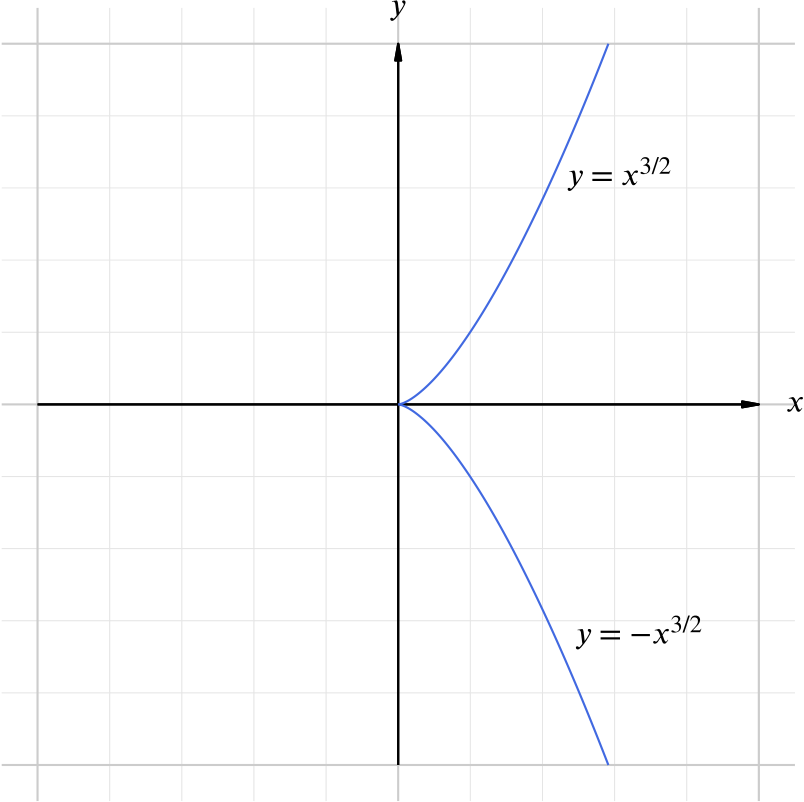
\includegraphics[width=0.5\textwidth]{img/y2x3}
\end{figure}

\begin{proposition}
    Let \(A\) be an integrally closed domain and \(K = \Frac(A)\). Let \(\alpha \in \overline{K}\) (= algebraic closure of \(K\). We can take the closure in any finite extension). We have \(A \subset K \subset \overline{K}\). Consider \(\alpha \in \overline{K}\).

    Then, \(\alpha\) is integral over \(A\) iff the minimal polynomial \(p_\alpha (x) \in K[x]\) of \(\alpha\) over \(K\) 
\end{proposition}

Note that minimal polynomial often depends on base field. For example, \(\sqrt[4]{2}\) has min poly \(x^4 - 2\) over \(\mathbb{Q}\) and \(x^2 - \sqrt{2}\) over \(\mathbb{Q} (\sqrt{2})\) 

\begin{proof}
    \(\impliedby\) by definition.

    \(\implies \): we have \(\alpha \) is integral.

    So, we have monic \(g(x)\in A[x]\) which is monic and \(g(\alpha) = 0\).

    Can we write \(g(x) = h(x) p_\alpha(x)\) in \(K[x]\)?

    Note that every root \(\beta\in \overline{K}\) of \(p_\alpha(x)\) is a root of \(g\). So, all roots of \(p_\alpha(x)\) are integral over \(A\).
    
    Note that coefficients of \(p_\alpha(x)\) are generated by the roots of the polynomial. The coefficients are the elementary symmetric polynomials.

    Thus, coefficients of \(p_\alpha\) lie in \(B \coloneqq \{ \alpha \in \overline{K} \mid \alpha \text{ is integral over } A \} \) 
    
    They also lie in \(K\)

    So, the coefficients are integral over \(A\) and in \(K\), hence in \(A\).

\end{proof}

Proposition 1.5 can be used to find \(\mathcal{O}_K\) for quadratic extension, \([K : \mathbb{Q} ] = 2\) (HW)

\subsection*{Preliminaries from the theory of fields}


In the following \(L / K\) will be a finite extension of fields.

\(L / K\) is called \underline{simple} if \(\exists \theta \in L\) such that \(L = K(\theta)\) 

\(L / K\) is called \underline{separable} if every \(\alpha \in L\) has a separable minimal polynomial over \(K\) [separable polynomial meaning no double roots in any extension field.]

For example, in \(K = \mathbb{F}_p(t)\) and \(L   = K(\sqrt[p]{t})\). Then \(p_{\sqrt[p]{t}}(x) = x^p - t = (x - \sqrt[p]{t})^p\) so not separable

\begin{theorem}
    [Theorem of the Primitive Element]
    
    If \(L / K\) is a finite separable extension, it is simple. 
\end{theorem}

\begin{definition}
    The \underline{trace} \(\operatorname{Tr}_{L / K} : L \to K \) and norm \(\N_{L / K}: L \to K\) are defined by:
    
        \(\Tr_{L / K}(x) = \Tr(T_x)\) 
        
        \(N_{L / L}(x) = \det (T_x)\) 

    Where \(T_x : L \to L\) is defined by \(T_x(y) = xy\) considered as an element of \(\End_K(L)\) 
\end{definition}

If \(n = [L : K]\) and \(f_x(t) = \det (t \operatorname{id}_L - T_x) = t^n + \alpha_1 t^{n-1} + \dots \) 

Then \(Tr _{L / K}(x) = -\alpha\) and \(N_{L / K}(x) = (-1)^n a_n\) 

Since \(T_{x+y} = T_x + T_y\) and \(T_{xy} = T_x \cdot T_y\) we have:

\(\Tr_{L / K}(x + y) = \Tr(T_{x+y}) = \Tr(T_x + T_y) = \Tr(T_x)+\Tr(T_y)=\Tr_{L / K}(x)+\Tr_{L / K}(y)\) 

\(N_{L / K}(xy) = \det(T_{xy})=\det(T_x T_y)=\det(T_x)\det(T_y)=N_{L / K}(x) N_{L / K}(y)\).

So, \(\Tr_{L / K}:L \to K\) is a homomorphism of vector spaces and \(N_{L / K}:L^\times \to K^\times\) is a homomorphism of the (product) group.

\begin{definition}
    Fix an algebraic closure \(\overline{L} \) of \(L\). A \underline{\(K\)-embedding} of \(L\) into \(E\) is a field homomorphism \(\sigma : L \to \overline{L}\) so tat \(\sigma(x) = x\) for all \(x\in K\).

    In other words, \(\sigma : L \to \overline{L} \) so that \(\sigma\) is \(K\)-linear.

    \(\Sigma (L / K)\) is the set of all such embeddings.
\end{definition}

Suppose \(L / K\) is simple and \(L = K(\theta)\). Let \(p_\theta (t)\in K[t]\) be the minimal polynomial of \(\theta\) over \(K\).

Then, the map from \(\Sigma (L / K)\) to the set of roots of the minimal polynomial \(\alpha \in \overline{L} \mid p_\theta (\alpha) = 0\) given by \(\sigma \mapsto \sigma(\theta)\) is a bijection.

In particular if \(L / K\) separable, then: \(\vert \Sigma (L / K) \vert = \deg(p_{\theta})=[L : K]\).

\begin{lemma}
Let \(L \) be finite and \(K \subset M \subset L\) an intermediate field. Then the restriction map \(\operatorname{res} : \Sigma (L / K) \to \Sigma (M / K)\) given by \(\operatorname{res}(\sigma) = \sigma \mid_M\)  is surjective.

Now suppose that \(\Sigma (M / K) \to \Sigma (L / K)\), given by \(\tau \mapsto \tilde{\tau}\), is any right inverse of \(\operatorname{res}\) [meaning, \(\tilde{\tau } \mid _M = \tau\)]. Then, for each \(\tau \in \Sigma(M / K)\), the map \(\operatorname{res}^{-1} (\tau) : \Sigma (L / K) \to \Sigma (\tilde{\tau}(L) / \tilde{\tau}(M))\) given by \(\sigma \mapsto [\tilde{\tau}(y) \mapsto \sigma(y)]\)  is bijective.\footnote{Here we consider \(\overline{L}\) as an algebraic closure of \(\tilde{\tau}(L) \subset L\).}
\end{lemma}

\begin{proof}
    Lorenz, \emph{Algebra}, Volume 1, chapter 7, section 1, Lemma.
\end{proof}

\begin{proposition}
    Let \(L / K\) be finite separable and \(x\in L\). Then,
    
    \begin{enumerate}[label=\roman*)]
        \item  \(f_x(t) = \det (t \id_L - T_x) = \prod_{\sigma \in \Sigma (L / K)}^{}(t - \sigma(x)) \)
        
        \item \(\Tr_{L / K}(x) = \Sigma_{\sigma \in \Sigma (L / K)} \sigma(x)\) 
        
        \item \(N_{L / K}(x) = \prod_{\sigma \in \Sigma (L / K)} \sigma (x)\) 
        
        \item If \(K \subset M \subset L\), then \(\Tr_{L / K} = \Tr_{M / K} \circ \Tr_{L / M}\) and \(N_{L / K} = N_{M / K} \circ N_{L / M}\). 

    \end{enumerate}  

\end{proposition}

\begin{proof}
    Neukirch, ch I, 2.6 and 2.7
\end{proof}

\begin{definition}
    Let \(L /K\) be finite separable extension and \(\alpha_1, \dots , \alpha_n\) be basis of \(L\) as a \(K\) vector space.

    Then the discriminant of \(\alpha_1, \dots ,\alpha_n\) is defined by:

    \(d(\alpha_1, \dots , \alpha_n) = \det(\sigma_i(\alpha_j))^2\) where \(\Sigma (L / K) = \{ \sigma_1, \dots , \sigma_n \} \) 
\end{definition}

\underline{Remark:} \(d(\alpha_1, \dots , \alpha_n)\) does not depend on the ordering of \(\alpha_1, \dots , \alpha_n\) and not on the chosen ordering of the elements in \(\Sigma(L / K)\) 

We now show that the \(d(\alpha_1, \dots , \alpha_n)\) is in \(K\). Let \(S\) be the matrix.

\[d(\alpha_1, \dots , \alpha_n) = \det(S)^2 = \det(S)\det(S^T) = \det (S^T S)\]

\[
    =\det \left[ \left[ \sum_{k} \sigma_k(\alpha_i)\sigma_k(\alpha_j) \right]_{ij}\right] = \det \left[ \left[ \sum_{k} \sigma_k(\alpha_i\alpha_j) \right]_{ij}\right]
\]
 
\[
    = \det \left[ (\Tr_{L / K} (\alpha_i \alpha_j) )_{ij} \right] 
\]

Since the trace is in \(K\), we see that the determinant must also be in \(K\).

\section*{Tuesday, 9/3/2024}

\subsection*{The Discriminant}

Let \(L / K\) be a finite separable field extension, and \((\alpha_1, \dots , \alpha_n)\) a basis of \(L / K\). Then,

\[
    d(\alpha_1, \dots , \alpha_n) = \det[(\sigma_i(\alpha_j))_{1 \le i,j \le n}]^2
\]

Where \(\Sigma(L / K) = \{ \sigma_1, \dots , \sigma_n \}\). Note that this is independent of order.

We have seen,

\[
    d(\alpha_1, \dots , \alpha_n) = \det \left[ (\Tr_{L / K}(\alpha_i \alpha_j))_{i j} \right] \in K
\]

In fact this is an alternate definition.

\begin{proposition}

    Let \(L / K\) be any (possibly inseparable) finite field extension. Then the \(K\)-bilinear form

    \[
        L \times L \to K, (x,y) = \Tr_{L / K}(xy)
    \]

is non-degenrate if and only if \(L / K\) is separable. In this case, \(d(\alpha_1, \dots , \alpha_n) \neq 0\) for any \underline{basis} \((\alpha_1, \dots , \alpha _n)\) of \(L / K\).

\end{proposition}


\begin{proof}
    Sketch \(\impliedby\): Let \(L = K(\theta)\). It can be proven [HW2] that
    
    \[
        d(1, \theta , \theta ^2, \dots , \theta^{n-1}) = \prod_{1 \leq i \neq j \leq n}^{} (\theta_i - \theta_j)^2
    \]
    
    where \(\theta_i\) are the conjugates of \(\theta\) in \(\overline{L}\).

    This finishes the proof.
\end{proof}

\underline{General Setting}: Let \(A\) be an integral domain, \(K = \Frac(A)\). Suppose \(L / K\) is a finite separable extension.

\(B \coloneqq \) integral closure of \(A\) in \(L\). Let \(C\) be the integral closure of \(A\) in \(\overline{L}\).

Assume in the following that \(A\) is integrally closed.

\underline{Observation}: If \(x\in B \subset C\) then \(\forall \sigma \in \Sigma (L / K), \sigma(x)\in C\).

Therefore, \(\Tr_{L / K}(x) = \Sigma_{\sigma \in \Sigma (L / K)} \sigma(x) \in C \cap K = A\) [since \(A\) is integrally closed.]

Similarly, \(N_{L / K}(x) = \prod_{\sigma \in \Sigma (L / K)}^{} \sigma (x) \in C\cap K = A\).

So, the norm and trace of elements of \(B\) are contained in \(A\). 

\underline{Remark}: If \(x\in B\), then \(x\in B^{\times} \iff N_{L / K} (x)\in A^\times\) 

\begin{proof}
    Suppose \(xy = 1\) for some \(y\in B \implies N_{L / K}(xy) = 1 \implies N_{L / K}(x) N_{L / K}(y) = 1\).

    For the other direction, \(N_{L / K}(x) = x \underbrace{\prod_{\sigma \neq \id}^{} \sigma(x)}_{b} = xb\). Note that \(b \in C \cap L = B\). 

    Since the norm is a unit, there exists \(a\in A \subset B\) such that \(axb = 1\). Therefore, \(x(ab) = 1 \implies x\in B^\times\).

\end{proof}

\begin{lemma}
    Let \((\alpha_1, \dots , \alpha_n)\) be a basis of \(L / K\) such that \(\alpha_i \in B\). Then,

    \[
        d(\alpha_1, \dots , \alpha_n) B \subset A \alpha_1 + \dots + A \alpha_n
    \]
\end{lemma}

\begin{proof}
    By 1.9, we may assume \(L / K\) is separable. Write an arbitrary element \(\alpha \in B\) as \(\alpha = a_1 \alpha _1 + \dots + a_n \alpha_n\) with \(a_i \in K\).

    Then, \(\Tr(\alpha_i \alpha) = \sum_{j=1}^{n} \Tr(\alpha_i \alpha_j)a_j = \begin{bmatrix}
        \Tr(\alpha_i \alpha_1) & \cdots &  \Tr(\alpha_i \alpha_n)  \\
    \end{bmatrix}\begin{bmatrix}
        a_1 \\
        \vdots \\
        a_n \\
   \end{bmatrix}\). Therefore,

   \[
    \begin{bmatrix}
        \Tr(\alpha_1 \alpha) \\
        \vdots \\
        \Tr(\alpha_n \alpha) \\
      \end{bmatrix}=\underbrace{[\overbrace{\Tr(\alpha_i \alpha_j)}^{\in A}]_{1 \leq i, j \leq n}}_{S} \begin{bmatrix}
             a_1 \\
             \vdots \\
             a_n \\
        \end{bmatrix}
   \]

    Multiplying on the left by \(S^{\ast}\) [the adjugate matrix of \(S\)],

    \[S^{\ast} S \begin{bmatrix}
         a_1 \\
         \vdots \\
         a_n \\
    \end{bmatrix} = S^{\ast} \begin{bmatrix}
         \Tr(\alpha_1 \alpha) \\
         \vdots \\
         \Tr(\alpha_n \alpha) \\
    \end{bmatrix}
    \] 

    \[\underbrace{\det(S)}_{d(\alpha_1, \dots , \alpha_n)} \begin{bmatrix}
        a_1 \\
        \vdots \\
        a_n \\
   \end{bmatrix} = \underbrace{S^{\ast}}_{\text{all entries are in } A} \begin{bmatrix}
        \Tr(\alpha_1 \alpha) \\
        \vdots \\
        \Tr(\alpha_n \alpha)\\
   \end{bmatrix} \in A^n
   \]

   Therefore, \(d(\alpha_1, \dots , \alpha_n)\alpha  = (\underbrace{d(\alpha_1, \cdots , \alpha_n) a_1}_{\in A}) \alpha_1 + \cdots + (\underbrace{d(\alpha_1, \cdots , \alpha_n) a_1}_{\in A})\alpha_n\) 

\end{proof}

\underline{Example}: Let \(K = \mathbb{Q} , L = \mathbb{Q}(\sqrt{5}), \alpha_1 = 1, \alpha_2 = \sqrt{5}\)

Then \(A = \mathbb{Z} , B = \mathbb{Z} \left[ \frac{1+\sqrt{5}}{2} \right] \) and \(d(1, \sqrt{5}) = \det \begin{bmatrix}
    1 &  \sqrt{5} \\
    1 &  -\sqrt{5} \\
\end{bmatrix} = 20\) 

Then, \(20 \cdot \mathbb{Z} \left[ \frac{1+\sqrt{5}}{2} \right] \subset \mathbb{Z} + \mathbb{Z} \sqrt{5} = \mathbb{Z} [\sqrt{5}] \) 

\underline{Remarks}:

\begin{enumerate}[label=\arabic*)] 

\item \(\forall \alpha \in L, \exists a \in A \setminus \{ 0 \}\) such that \(a \alpha \in B\).

\begin{proof}
    Suppose minimal polynomial of \(\alpha \) over \(K\) is \(p_\alpha (x) = x^d + a_1 x^{d-1} + \dots + a_d \in K[x] \implies \exists a \in A \setminus \{ 0 \} \) such that \(a a_i \in A, 1 \leq i \leq d\).

    Thus, \((ax)^d + \underbrace{a_1 a}_{\in A}(ax)^{d-1} + \cdots + \underbrace{(a^d a_d)}_{\in A}\).

    Thus, \(a \alpha\) is integral. Therefore, \(a \alpha \in B\)
\end{proof}

    \item \(\operatorname{span}_K(B) = L \)
    \item \(\Frac(B) = L\)  

\end{enumerate}

\begin{definition}
    An \(n\)-tuple \((\omega_1, \cdots, \omega_n)\in B^n\) is called an \underline{integral basis} of \(B\) over \(A\) if \(B = \bigoplus_{i=1}^n A \omega_i\)
\end{definition}

\underline{Remark}: If \((\omega_1, \dots , \omega_n)\) is an integral basis of \(B\) over \(A\), then it is a basis of \(L / K\) and hence \(n = [L : K]\).

Note that integral basis is \underline{not guaranteed} to exist.

\begin{proposition}
    If \(L / K\) is finite separable and \(A\) is a PID, then every finitely generated \(B\)-submodule \(M \neq 0\) of \(L\) is a free \(A\)-module of rank \([L : K]\).

    In particular, \underline{\(B\) has an integral basis over \(A\).} [Apply the proposition to \(M = B\)].
\end{proposition}

\begin{proof}
    Write \(M = \sum_{i=1}^{s} B \alpha_i\) with \(\alpha_i \in L^\times\). By the remark 1 above, we can find \(a \in A \setminus \{ 0 \} \) such that \(a \alpha_i \in B\) for \(1 \leq i \leq s\).

    Therefore, \(a \cdot M \subset B\). Since \(\underset{ax \leftarrow x}{aM \cong M} \) [as \(A\)-module], we may assume \(M \subset B\). 
    
    Therefore, \(\alpha_1 B = \underset{\neq 0}{B \alpha_1} \subset M \subset B\). (1)

    \underline{Fact} (from M502): Let \(A\) be a PID. Then every submodule \(N\) of a finitely generated free \(A\)-module \(F\) is free, and \(\rank_A(N) \leq \rank_A(F)\).

    Applying the fact to (1), it suffices to show that \(B\) is free of rank \(n\) over \(A\).

    Choose a basis \((\alpha_1, \cdots, \alpha_n)\) of \(L / K\) with all \(\alpha_i \in B\).
    
    By 1.10, \(d(\alpha_1, \dots , \alpha_n) B \underset{(2)}{\subset} A \alpha_1 + \cdots + A \alpha_n \underset{(3)}{\subset} B\) 

    Since \((\alpha_1, \cdots, \alpha_n)\) is a basis of \(L / K\), \(A \alpha_1 + \cdots + A \alpha_n\) is finitely generated free \(A\)-module of rank \(n\).
    
    (2) and fact together imply that \(d(\alpha_1, \cdots, \alpha_n) B\) is free of \(\rank \leq n\) over \(A\), and it is nonzero by 1.9.

    But \(B \to d(\alpha_1, \cdots, \alpha_n)B\), \(x \mapsto d(\alpha_1, \cdots, \alpha_n)x\), is an isomorphism of \(A\)-modules.
    
    (3) and fact together imply that \(B\) has rank \(\geq n\). 

    Therefore, \(\rank_A(B) = n\).

\end{proof}

\underline{Remark}: If \(L = K(\alpha)\) and \(p(x) = p_\alpha(x) \in K[x]\) is the minimal polynomial of \(\alpha\) over \(K\).

Let \(\alpha = \alpha_1, \cdots, \alpha_n\) be the roots of \(p_\alpha\) in \(\overline{L}\), counted with multiplicity.

Then, \(d(1, \alpha, \alpha^2, \cdots, \alpha^{n-1}) = \prod_{i < j}^{} (\alpha_i - \alpha_j)^2 = \operatorname{disc}(p_\alpha(x))\)

Recall that \(\operatorname{disc}(p) = \operatorname{resultant}(p, p^{\prime}) \).

\begin{definition}
    Let \(K\) be a number field and \(n = [K : \mathbb{Q}]\).

    \begin{enumerate}[label=\arabic*)]
        \item If \(0 \neq I \subseteq K\) is a finitely generated \(\mathcal{O}_K\)-module and \((\alpha_1, \cdots, \alpha_n)\) a basis of \(I\) as a \(\mathbb{Z}\)-module (exists by 1.11), then \(d(I) \coloneqq d(\alpha_1, \cdots, \alpha_n)\) is called the \underline{discriminant} of \(I\).
        \item \(d_K = d(\mathcal{O}_K)\) is called \underline{the discriminant of \(K\)}.
    \end{enumerate} 

\end{definition}

\underline{Remarks}:

\begin{enumerate}[label=\arabic*)]
    \item \(\mathbb{Z}\) is a PID \(\overset{1.11}{\implies}\) every \(I\) as in \((1)\) is indeed free of rank \(n = [K : \mathbb{Q}]\) over \(\mathbb{Z}\).
    \item \(d(I)\) doesn't depend on the choice of a basis. If \((\beta_1, \cdots, \beta_n)\) is another basis \(I\) over \(\mathbb{Z}\), then we can find a matrix \(M \in M_n(\mathbb{Z})\) such that \(M \begin{bmatrix}
         \alpha_1 \\
         \vdots \\
         \alpha_n \\
    \end{bmatrix} = \begin{bmatrix}
         \beta_1 \\
         \vdots \\
         \beta_1 \\
    \end{bmatrix}\). Note that \(M\)  must be invertible in \(M_n(\mathbb{Z})\) since we can also express the elements of the first basis as linear combination of the elements of the second basis with integral coefficients. Therefore, \(\det(M) \in \{ \pm 1 \}\).

    Therefore, \(\det(\beta_1, \cdots, \beta_n) = \det(M)^2 d(\alpha_1, \cdots, \alpha_n) = d(\alpha_1, \cdots, \alpha_n)\).
\end{enumerate}

\section*{Thursday, 9/5/2024}

\underline{Example}: \(K = \mathbb{Q} (i) \implies \mathcal{O}_K = \mathbb{Z}  + \mathbb{Z} i \implies d_K = \det \begin{bmatrix}
    1 &  i \\
    1 &  -i \\
\end{bmatrix}^2 = -4\).

Note: \(K = \mathbb{Q} (\sqrt{d_K})\). If \([K : \mathbb{Q}] = 2\) then \(K = \mathbb{Q}(\sqrt{d_K} )\) [Exercise]

\begin{proposition}
    Let \(0 \neq I \subset J\) be finitely generated \(\mathcal{O}_K\)-submodules of \(K\). Then,
    
    \[
        d(I) = [J : I]^2 d(J)
    \]
\end{proposition}

\begin{proof}
    Let \(I = \mathbb{Z} \alpha_1 \oplus \cdots \oplus \mathbb{Z} \alpha_n\) and \(J = \mathbb{Z} \beta_1 \oplus \cdots \oplus \mathbb{Z} \beta _n\). Then, there exists \(M \subset M_n(\mathbb{Z})\) such that \(M \begin{bmatrix}
         \beta_1 \\
         \vdots \\
         \beta_n \\
    \end{bmatrix} = \begin{bmatrix}
         \alpha_1 \\
         \vdots \\
         \alpha _n \\
    \end{bmatrix}\). 
    
    Then, \(d(I) = d(\alpha_1, \cdots , \alpha_n) = \det(M)^2 d(\beta_1, \cdots , \beta_n) = \det(M)^2 d(J)\). 
    
    To finish the proof, note that \(J / I \cong \mathbb{Z}^n / M(\mathbb{Z}^n) \cong \mathbb{Z}/(m_1) \oplus \cdots \oplus \mathbb{Z}/(m_n) \implies \vert m_1 \cdots m_n \vert = \vert \det(M) \vert = [J : I]\).

\end{proof}

\begin{corollary}
    If \(0 \neq I \subset \mathcal{O}_K\) is an ideal and \(d(I)\) is square-free, then \(I = \mathcal{O}_K\). If \(\theta \in \mathcal{O}_K\) and \(K = \mathbb{Q}(\theta)\), then \(d(1, \theta , \theta^2, \cdots , \theta^{n-1})\) is square-free, then \(\mathbb{Z}[\theta] =  \mathcal{O}_K\).  
\end{corollary}

\begin{proof}
    \(d(I)\) is square free.
    
    \(1.12 \implies d(I) = [\mathcal{O}_K : I]^2 d(\mathcal{O}_K)\), which is only possible when \([\mathcal{O}_K : I] = 1\).
    
    Suppose \(\mathcal{O}_K = \mathbb{Z} \alpha_1 \oplus \cdots \oplus \mathbb{Z} \alpha_n\) and \(M \in M_n(\mathbb{Z})\) such that \(M \begin{bmatrix}
         \alpha_1 \\
         \vdots \\
         \alpha_n \\
    \end{bmatrix} = \begin{bmatrix}
         1 \\
         \vdots \\
         \theta^{n-1} \\
    \end{bmatrix}\). 

    It follows that \(d(1, \theta , \cdots , \theta^{n-1}) = \det(M)^2 d(\alpha_1, \cdots , \alpha_n)\), implying \(\det(M)^2 = 1\implies \det(M) = \pm 1\). 

    Therefore \(\begin{bmatrix}
         \alpha_1 \\
         \vdots \\
         \alpha_n \\
    \end{bmatrix} = M ^{-1} \begin{bmatrix}
         1 \\
         \vdots \\
         \theta^{n-1} \\
    \end{bmatrix} \implies \mathbb{Z}[\theta] = \mathcal{O}_K\). 
\end{proof}


\chapter{Ideals}

Suppose \(K\) is a number field, and \(\mathcal{O} = \mathcal{O}_K\).

\begin{definition}
    An element \(\alpha \in \mathcal{O} \setminus \{ 0 \} \) is called \underline{irreducible} if \(\alpha\) is not a unit \([\alpha \notin \mathcal{O} ^\times]\) and whenever \(\alpha = \beta \gamma\) with \(\beta , \gamma \in \mathcal{O}\) then either \(\beta \in \mathcal{O} ^\times \) or \(\gamma \in \mathcal{O} ^\times \) 
\end{definition}

This is not the same as the definition of a prime element. In general, irreducible elements may not be prime elements (which are those non-zero elements which generate prime ideals).

\underline{Observation}: Every \(0 \neq \alpha \in \mathcal{O}  \setminus \mathcal{O} ^\times\) can be expressed as a product of irreducible elements.

\begin{proof}
    If \(\alpha\) is irreducible, there's nothing to do.

    If it is not irreducible, then \(\alpha = \beta \gamma\) with \(\beta, \gamma\) both non-units.

    Using the remark before 1.10, \(\vert N_{K / \mathbb{Q}}(\beta) \vert > 1\) and \(\vert N_{K / \mathbb{Q}}(\gamma) \vert > 1\).

    Moreover, \(\vert N_{K / \mathbb{Q}}(\alpha) \vert > \vert N_{K / \mathbb{Q}}(\beta) \vert, \vert N_{K / \mathbb{Q}(\gamma)} \vert\). 

    By applying \underline{strong induction} on \(\vert N_{K / \mathbb{Q}}(\alpha) \vert\), we see that \(\beta \) and \(\gamma\) can be written as products of irreducibles. Thus, \(\alpha\) can be written as a product of irreducibles.  
\end{proof}

\textbf{Example}: \(K = \mathbb{Q} (\sqrt{-5}), \mathcal{O}_K = \mathbb{Z} [\sqrt{-5}]\). Here,

\[
    21 = 3 \cdot 7 = (1 + 2 \sqrt{-5})(1 - 2 \sqrt{-5})
\]

HW2: \(3, 7, 1 + 2 \sqrt{-5}, 1 - 2 \sqrt{-5}\) are all irreducibles and are pairwise non-associates.

\(\implies\) factorization into irreducibles is \underline{not} unique.

[This is equivalent to the fact that not every irreducible element is a prime element.]

\underline{Conclusion}: \(\mathcal{O}_K\) is not a UFD in general!

\begin{theorem}
    The ring \(\mathcal{O}_K\) is noetherian, integrally closed and every non-zero prime ideal is maximal [\(\iff \) Krull dimension of \(\mathcal{O}_K\) is \(1\)].
\end{theorem}

\begin{proof}
    \underline{\(\mathcal{O}_K\) is noetherian}: if \(0 \neq I \subset \mathcal{O}_K\) is an ideal \(\overset{1.11}{\implies} I\) is a finitely generated as a \(\mathbb{Z}\)-module \(\implies I\) is finitely generated as an \(\mathcal{O}_K\)-module.
    
    \underline{\(\mathcal{O}_K\) is integrally closed}: remark after 1.4.

    \underline{Non-zero prime ideals are maximal}: Suppose \(0 \neq P \subset \mathcal{O}_K\) is a non-zero prime ideal.
    
    \(\overset{1.12}{\implies} [\mathcal{O}_K : P]\) is finite. In fact, \(d(P) = [\mathcal{O}_K : P]^2 d(\mathcal{O}_K)\).
    
    Hence, \(\mathcal{O}_K / P\) is a finite integral domain. But finite integral domains are fields.

    Thus, \(\mathcal{O}_K / P\) is a field, and thus \(P\) is maximal.

\end{proof}

This gives us the inspiration to define Dedekind domain.

\begin{definition}
    An integral domain \(A\) is called \underline{Dedekind domain} if:

    \begin{enumerate}[label=\arabic*)]
        \item \(A\) is noetherian.
        \item \(A\) is integrally closed.
        \item Every non-zero prime ideal \(P\) of \(A\) is maximal. 
    \end{enumerate} 
\end{definition}

By Theorem 2.1, \(\mathcal{O}_K\) is a \underline{Dedekind domain}.

Moreover, we have:

\begin{enumerate}[label=\arabic*)]
    \item \(k[x]\) when \(k\) is a field is a Dedekind domain.
    \item \(\mathbb{C}[x,y] / (y^2 - x^3)\) is \underline{not} a Dedekind domain. It fails the integrally closed condition, as we saw earlier. 
\end{enumerate} 

From now on, \(\mathcal{O}\) denotes a Dedekind domain.

\begin{definition}
    \(\operatorname{Id}(\mathcal{O}) =\) set of ideals of \(\mathcal{O}\).

    \(\operatorname{Id^\times}(\mathcal{O}) = \operatorname{Id}(\mathcal{O} ) \setminus \{ (0) \}\).

    \(\operatorname{Max}(\mathcal{O}) =\) set of maximal ideals of \(\mathcal{O} \). 
\end{definition}

\begin{lemma}
    \(\forall I \in \operatorname{Id^\times }(\mathcal{O}) \), there exists primes \(P_1, \cdots , P_r \in \operatorname{Max}(\mathcal{O}) \) such that \(P_1 \cdots P_r \subset I\).
\end{lemma}

\begin{proof}
    Suppose \(X = \{ J \in \operatorname{Id^\times }(\mathcal{O}) \mid J \text{ does not contain a product of maximal ideals} \} \)
    
    Note that \(X\) does not contain \(\mathcal{O} = (1)\) since it \(X\) contains all the prime ideals.

    \underline{Goal}: We want to show that \(X = \varnothing\). Suppose \(X\) is non-empty. Since \(\mathcal{O}\) is noetherian, we cannot have infinite ascending chains.

    Using the fact that \(X\) is partially ordered by \(\subset\), \(X\) contains maximal elements. Let \(I \in X\) be a maximal element.

    Since \(I\in X\), \(I\) is not a prime. Which means, we can find \(x,y\notin I\) such that \(xy\in I\).
    
    Set \(I_1 \coloneqq (x)+I\) and \(I_2 \coloneqq (y)+I\).

    Then, \(I_1\) and \(I_2\) contain \(I\). Since \(I\) is maximal, \(I_1, I_2\notin X\).

    This means we can find \(P_1, \cdots , P_m\) and \(Q_1, \cdots, Q_{m^{\prime}}\) such that \(\prod_{i=1}^m P_i \subset I_1\) and \(\prod_{j=1}^{m^{\prime}} Q_j \subset I_2\).

    Then, \(\prod_i P_i \prod_j Q_j \subset I_1 I_2 = ((x)+I)((y)+I)\), since \(xy\in I\) we have \(I_1 I_2 \subset I\). 

\end{proof}

\begin{lemma}
    Suppose \(P \in \operatorname{Max}(\mathcal{O})\) and \(P ^{-1} = \left\{ x \in \underset{=\Frac(\mathcal{O})}{K} \mid xP \subset \mathcal{O} \right\} \) [this is an \(\mathcal{O}\)-submodule of \(K\), containing \(\mathcal{O}\)]
    
    Then, \(\forall I \in \operatorname{Id^\times}(\mathcal{O}), I P ^{-1} \supsetneq I\).
\end{lemma}

\begin{proof}
    \underline{Step 1}: We sow \(P ^{-1} \supsetneq \mathcal{O}\). Suppose \(c \in P \setminus \{ 0 \} \).

    \(2.2 \implies \exists P_1, \cdots , P_r \in \operatorname{Max}(\mathcal{O}) \) such that \(P_1 \cdots P_r \subset (c) = c \cdot \mathcal{O} \subset P\)

    Assume that \(r\) is minimal with this property.

    Recall that, if ideal product \(IJ \subset P\) then \(I \subset P\) or \(J \subset P\).

    Therefore, there exists \(i\) such that \(P_i \subset P\). Since \(P_i\) is also a maximal ideal, \(P_i = P\).

    This means the chain of subsets are all equalities. By reordering the prime ideals, we may assume \(i = 1\).

    Since \(r\) is minimal, \(P_2 P_3 \cdots P_r \not \subset (c)\).
    
    This implies there exists \(b \in P_2, \cdots , P_r \setminus (c)\) such that \(\underset{\in K}{\dfrac{b}{c}} \notin \mathcal{O} \). However,

    \[
        \frac{b}{c} \cdot P = \frac{b}{c} \subset P_1 \subset \frac{1}{c} P_2 \cdots P_r P_1 \subset \frac{1}{c}(c) = \mathcal{O}
    \]

    Therefore, \(\frac{b}{c} \in P ^{-1} \setminus \mathcal{O} \implies P ^{-1} \supsetneq \mathcal{O}\).

    \underline{Step 2}: We'll show: \(I P ^{-1} \supsetneq I\) where \(I \neq (0)\).

    Write \(I = \sum_{i=1}^{m} \mathcal{O} \alpha_i\) where \(\alpha_i \neq 0\).

    Suppose \(I P ^{-1} = I \implies \) if \(x \in P ^{-1}\), then \(x \alpha _i = \sum_{j=1}^{m} a_{ij} \alpha_j\).

    Set \(A \coloneqq \left[ x \partial _{ij} - a_{ij} \right] _{1 \leq i, j \leq m}\). Then, \(A \begin{bmatrix}
         \alpha_1 \\
         \vdots \\
         \alpha _m \\
    \end{bmatrix} = \begin{bmatrix}
         0 \\
         \vdots \\
         0 \\
    \end{bmatrix}\). Multiplying on the left by \(A^{\ast}\) we see  that,

    \[
        \det (A) \begin{bmatrix}
             \alpha_1 \\
             \vdots \\
             \alpha_m \\
        \end{bmatrix} = \begin{bmatrix}
             0 \\
             \vdots \\
             0 \\
        \end{bmatrix} \implies \forall i, \det(A) \alpha_i = 0 \implies \det (A) = 0
    \]

    Since \(\det (A)\) is a monic polynomial, we deduce that \(x\) is integral over \(\mathcal{O}\), which means \(x\in \mathcal{O}\). Therefore, \(P ^{-1} \subset \mathcal{O}\). This is a contradiction.

    Therefore, \(I P ^{-1} \supsetneq I\).
\end{proof}

\begin{theorem}[Unique Factorization in Dedekind Domain]
    Every \(I \in \operatorname{Id^\times}(\mathcal{O}) \) can be written as:

    \[
        I = P_1 P_2 \cdots P_r
    \]

    with \(P_1, \cdots , P_r \in \operatorname{Max}(\mathcal{O})\), and this factorization is unique upto ordering. 
\end{theorem}

\section*{Tuesday, 9/10/2024}

\begin{proof}

    Step 1, Existence:

    Let \(X = \{ J \in \operatorname{Id^\times }(\mathcal{O}) \mid J \text{ does not have a factorization into prime ideals} \} \). We want to show that \(X = \varnothing\).

    Assume \(X \neq \varnothing\). \(\mathcal{O}\) is a dedekind domain, and thus it is noetherian. Therefore, \(X\) has a maximal element \(I\).

    \(I \neq \mathcal{O}\) [since \(\mathcal{O} \notin X\)].

    Thus, there is a maximal ideal \(P\) containing \(I\).

    Since \(I\in X\), \(I \neq P\). Therefore, \(P\supsetneq I\).

    By lemma 2.3, \(I P ^{-1} \supsetneq I\).

    Again, by lemma \(2.3\), \(P ^{-1} P \supsetneq P\), \(P ^{-1} P\) is an ideal \(\subsetneq \mathcal{O}\). Therefore, by the maximality of \(P\), we see that \(P ^{-1} P = \mathcal{O}\).
    
    Now, suppose \(\mathcal{O} = I P ^{-1} \). Multiplying both sides by \(P = I P ^{-1} P = I\), which is a contradiction.
    
    Thus, \(I \subsetneq I P ^{-1} \subsetneq \mathcal{O}\).

    Now, since \(I\) is a maximal element of \(X\), \(I P ^{-1} \notin X\).

    Thus, we can find maximal ideals \(P_1, \cdots , P_r\) so that \(I P ^{-1} = P_1 \cdots P_r\).

    Multiplying both sides by \(P\), we see that,

    \(I = I P ^{-1} P = P_1 \cdots P_r P \) which is a contradiction.

    Thus, \(X\) must be empty. This shows existence.

    Uniqueness: HW.

\end{proof}

\begin{theorem}
    [Chinese Remainder Theorem]

    Let \(I_1, \cdots , I_r\) be ideals of a ring \(R\) which are pairwise co-prime [i.e. \(I_i + I_j = R \quad \forall i \neq j\)]. Then,
    
    \begin{enumerate}[label=\roman*)]
        \item \(I_1 \cdots I_r = \bigcap_{j=1}^{r} I_j\)  
        \item The canonical map \(R / \bigcap_{j=1}^{r} I_j \to \prod_{j=1}^{r} R / I_j\) sending \(a + \bigcap_{j=1}^{r} I_j \mapsto (a + I_j)^r_{j=1}\) is a ring isomorphism.
    \end{enumerate} 

\end{theorem}

\begin{proof}
    Neukirch 3.6, Atiyah-MacDonald
\end{proof}

\begin{definition}
    Let \(\mathcal{O}\) be a Dedekind domain, and \(K = \Frac(\mathcal{O})\). Then, a \underline{fractional ideal} of \(K\) is a non-zero finitely generated \(\mathcal{O}\)-submodule of \(K\).
    
    For any \(a \in K^\times\), we call \(a \cdot \mathcal{O}\) a \underline{principal fractional ideal}.
    
    The non-zero ideals of \(\mathcal{O}\) are called \underline{integral ideals}.

    We denote by \(\mathcal{J}_K\) the set of fractional ideals of \(K\), and by \(\mathcal{P}_K\) the set of principal fractional ideals.

\end{definition}

\begin{example}
    \(\frac{1}{2}\mathbb{Z}\) is a fractional ideal for \(\mathcal{O} = \mathbb{Z}\). 
\end{example}

\underline{Observation}: Let \(I \subset K\) be a non-zero \(\mathcal{O}\)-submodule.

Then \(I\) is fractional of \(K \iff \exists c\in \mathcal{O} \setminus \{ 0 \}\) such that \(c \cdot I \subset \mathcal{O}\).

\begin{proof}
    If it is a fractional ideal of \(K\), it is finitely generated as an \(\mathcal{O} \)-module. Suppose it is generated by \( \frac{a_1}{s_1}, \dots, \frac{a_r}{s_r}   \) for nonzero \(s_1, \cdots , s_r \in \mathcal{O}\). We can set \(c = s_1 \cdots s_r\) which gives us \(c \cdot I = 0\).

    For the other direction, suppose \(c \cdot I \subsetneq \mathcal{O}\). Since \(\mathcal{O}\) is noetherian, it is finitely generated as an \(\mathcal{O}\)-module.

    Therefore, \(I = \frac{1}{c}(cI)\) is also finitely generated as an \(\mathcal{O}\)-module. Thus, \(I\) satisfies all the conditions of being a fractional ideal, and thus is a fractional ideal by definition. 

\end{proof}

\begin{proposition}
    [Definition of Ideal Group] The fractional ideals of \(K\) form an abelian group w.r.t.\ multiplication, which is called the \underline{ideal group} of \(K\).
    
    The identity element is \((1) = \mathcal{O}\).

    Inverse is given by \(I ^{-1} = \{ x \in K \mid xI \subsetneq \mathcal{O} \} \) 
\end{proposition}

\begin{proof}
    First we prove that the product of two fractional ideals are fractional ideals.

    \(I, J \subset \mathcal{J}_K \implies cI \subset \mathcal{O}, dJ \subset \mathcal{O}\). Therefore, \((cd)IJ = (cI)(dJ) \subset \mathcal{O}\). Therefore, \(IJ \subset \mathcal{J}_K\).

    Commutatitivty and associativity follows from \(\mathcal{O}\) itself being a commutative ring.

    We need to prove the existence of inverses. Idea: \((P_1 \cdots P_r) ^{-1} = P_1 ^{-1} \cdots P_r ^{-1}\) 

    Given \(I \subset \mathcal{J}_K, \exists c \in \mathcal{O} \setminus \{ 0 \} \) such that \(cI \subseteq \mathcal{O} \).

    We can factor \(cI\) into primes. Thus, \(cI = P_1 \cdots P_r\).

    For any \(J \in \mathcal{J}_K\), we define \(\overline{J} = \{ x \in K \mid xJ \subseteq \mathcal{O} \} \).

    Note that, if \(d\in J \setminus \{ 0 \}\), we have \(d \overline{J} \subseteq \mathcal{O}\).

    Furthermore, \(d \overline{J} \) is finitely generatd implies \(\overline{J} = \frac{1}{d} = \frac{1}{d}(d \overline{J})\) is finitely generated as a \(\mathcal{O}\)-module. 
    
    Thus, \(\overline{J} \in \mathcal{J}_K\).

    Going back to \(I\), we see that \((c) \overline{P_1} \cdots \overline{P_r} I = \overline{P_1} \cdots \overline{P_r} (cI) = (\overline{P}_1 P_1) \cdots (\overline{P_r} P_r) = \mathcal{O} \cdots \mathcal{O} = \mathcal{O}\).  

    Thus, \(\forall J \in \mathcal{J}_K, \exists J ^{-1} \in \mathcal{J}_K\) such that \(J ^{-1} \cdot J = J \cdot J ^{-1} = \mathcal{O}\).

\end{proof}

\begin{corollary}
    Every \(I \in \mathcal{J}_K\) has a factorization:

    \[
        I = P_1 ^ {e_1} \cdots P_r^{e_r}
    \]

    where \(P_1, \cdots , P_r\) are pairwise distinct prime/maximal ideals and \(e_1, \cdots , e_r\) are uniquely determiend integers.

    As usual, if \(e < 0\) then \(J^e \coloneqq (J ^{-1} )^{-e}\) for any \(J \in \mathcal{J}_K\).

\end{corollary}

\begin{proof}
    Choose \(c \in \mathcal{O} \setminus \{ 0 \} \) so that \(cI \subset \mathcal{O} \implies cI = P_1^{a_1}\cdots P_r^{a_r}\) with \(a_i \geq 0\).

    Also write \(c \mathcal{O} = P_1^{b_1}\cdots P_r^{b_r}\) with \(b_i \geq 0\).

    Exponent of \(0\) are allowed to make sure the primes are the same.

    Therefore, \(I = (c)^{-1} (cI) = P_1^{a_1 - b_1} \cdots P_r^{a_r - b_r}\) 

    Uniqueness is HW.

\end{proof}

Note that, in the group of (fractional) ideals, the principal ideals form a subgroup.

\begin{definition}
    The \underline{ideal class group} of \(K\) is defined as \(\mathcal{J}_K / \mathcal{P}_K\) and denoted by \(\Cl_K\). We call \(h_K = \vert \Cl_K \vert \) the \underline{class number} of \(K\).
\end{definition}

We have the exact sequences:

\[
    1 \to \mathcal{P}_K \to \mathcal{J}_K \to \Cl_K \to 1
\]

\[
    1 \to \mathcal{O} ^\times \to \underset{c}{K^\times} \underset{\mapsto}{\to} \underset{c \mathcal{O}}{\mathcal{P}_K} \to 1
\]

\underline{Remark}: \(\mathcal{O}\) is a PID \(\iff \Cl_K = \{ 1 \}\)

\begin{proof}
    Suppose \(I\) is a fractional ideal. Then, \(cI\) is an ideal for some \(c\). Since \(\mathcal{O}\) is a PID, we see that \(cI\) is a principal ideal, so \(cI = (d)\). Therefore, \(I = \frac{d}{c} \mathcal{O}\). Thus, \(\mathcal{J}_K = \mathcal{P}_K \implies \Cl_K = \{ 1 \}\).

    For the other direction, suppose \(\Cl_K = \{ 1 \}\). Then, \(\mathcal{J}_K = \mathcal{P}_K\). Given \(I \in \operatorname{Id^\times }(\mathcal{O})\) there exists \(c\in K^\times\) such that \(I = c \mathcal{O}\). Since \(c\in I\) we see that \(I\) is a principal ideal. 
\end{proof}

Note that \(\Cl_K\) being trivial is also equivalent to \(\mathcal{O}\) being a UFD.

The main results of the first part of the course are: if \(K\) is a number field,

\begin{itemize}
    \item The finiteness of the class number
    \item Dirichlet's Theorem on Units.
    
    \(\mathcal{O}_K^\times \cong \mathbb{Z}^{r + s - 1} \oplus \{ \text{roots of unity in \(K\)}  \} \)
    
    Where \(r\) is the number of real embeddings 
    
    \(r = \vert \{ K \hookrightarrow \mathbb{R} \}  \vert \).
    
    And \(2s\) is the number of complex embeddings which do not factor through \(\mathbb{R} \)
    
    \(2s = \vert \{ K \underset{\mathbb{Q}}{\hookrightarrow} \mathbb{C} \text{ does not factor through } \mathbb{R} \}  \vert \).
\end{itemize} 

\subsection*{Decomposition of primes in \(\mathcal{O}_K\)}

c.f. Neuker, ch I

Here, \(K =\) number field, \(\mathcal{O} = \mathcal{O}_K, n = [K : \mathbb{Q}]\).

\begin{definition}
    Given a prime number \(p \in \mathbb{Z}_{> 0}\) we write \(p \cdot \mathcal{O}_K = P_1^{e_1} \cdots P_r^{e_r} \quad (\ast)\) with pairwise distinct maximal ideals $P_i$. \(p\) is called:

    \begin{enumerate}[label=\roman*)]
        \item \underline{unramified} (in \(K\)) if \(e_1 = \cdots = e_r = 1\).
        \item \underline{ramified} (in \(K\)) if \(\exists 1 \leq i \leq r : e_i > 1\).
        \item \underline{completely split} (\underline{totally split}, \underline{totally demomposed}) if it is unramified and \(r = n\).
        \item \underline{inert} if \(r = 1, e_1 = 1\).
    \end{enumerate} 
\end{definition}

\begin{example}
    Suppose \(K = \mathbb{Q} (i)\), then \(\mathcal{O}_K = \mathbb{Z} [i]\) and \(2 \cdot \mathbb{Z} [i] = (1+i)^2\) so \(2\) ramified.

    If \(p \equiv 1 \pmod 4\) then \(p \mathbb{Z} [i] = P_1 P_2\) with \(P_1 \neq P_2\) maximal ideals, so \(p\) is completely split [and also unramified].
    
    If \(p \equiv 3 \pmod 4\) then \(p \mathbb{Z} [i]\) is a maximal ideal, therefore \(p\) is inert.

\end{example}

\underline{Fundamental Questions}: Given \(K\), how can we characterize

\[
    \operatorname{Spl}_K = \{ p \in \mathbb{Z} _{>0} \text{ is prime} \mid p \text{ is totally split in } K \} \,?
\]

In \(\mathbb{Q} (i)\) we have a rule: \(p \equiv 1 \pmod 4\) if and only if \(p\) is totally split. For quadratic extensions we have similar rules. More generally, if the Galois closure of $K$ over $\mathbb{Q}$ has an abelian Galois group over $\mathbb{Q}$, then $\operatorname{Spl}_K$ can be described using congruence conditions.

If the Galois group of (the normal closure of) $K$ over $\mathbb{Q}$ is not abelian, one can sometimes use modular forms or Maass forms to describe $\operatorname{Spl}_K$. In general, the \emph{Langlands Program} predicts that one can use automorphic representations to describe $\operatorname{Spl}_K$.

\section*{Thursday, 9/12/2024}

Recall that,

\[
    \operatorname{Spl}_K = \{ p \in \mathbb{Z} _{>0} \mid p \text{ is totally split in } K \}
\]

\begin{example}
    \(\operatorname{Spl}_{\mathbb{Q}(\sqrt{-3})} = \{ p \text{ prime } \mid p\equiv 1 \pmod 3 \} \)

    \(\operatorname{Spl}_{\mathbb{Q} (\sqrt[3]{2})} = \{ p \text{ prime } \mid \exists x,y\in \mathbb{Z} \times \mathbb{Z} : p = x^2 +27y^2 \}  \) 

\end{example}

We can write:

\[
    p \mathcal{O} _K = P_1^{e_1} \cdots P_r^{e_r} \text{ with pairwise distinct } P_i\in \operatorname{Max} (\mathcal{O} _K), e_i > 0 \quad(\ast)
\]

\underline{Question}: How does one find a decomposition \((\ast)\)?

\begin{definition}[Conductor]
    Let \(\theta \in \mathcal{O} = \mathcal{O}_K\) such that \(K = \mathbb{Q} (\theta)\).Then,

    \[
        C = \{ \alpha \in \mathcal{O} \mid \alpha \mathcal{O} \subset \mathbb{Z} [\theta] \} 
    \]

    \(C\) is called the \underline{conductor} of \(\mathbb{Z} [\theta]\).

    This is an ideal in \(\mathcal{O}\). 

    \underline{Note}: 1.10 implies, \(d(1, \theta , \cdots , \theta^{n-1})\cdot \mathcal{O} \subset \mathbb{Z} + \mathbb{Z} \theta + \cdots + \mathbb{Z} \theta ^{n-1} = \mathbb{Z} [\theta]\) where \(n = [K : \mathbb{Q}]\). Thus, \(d(1, \theta , \cdots , \theta^{n-1}) \in C \implies C \neq 0\)  

    \underline{Note}: \(Q\in \operatorname{Max} (\mathbb{Z} [\theta])\) so that \(Q\) is not invertible in \(\mathbb{Z}[\theta] \iff C \subset Q\). \(C\) is the largest ideal of \(\mathcal{O}_K\) such that: if \(Q \in \operatorname{Max}(\mathbb{Z}[\theta])\) is not invertible in \(\mathbb{Z} [\theta] \iff C \subset Q\).   

\end{definition}

\begin{definition}[Norm of an Ideal]
    If \(I \in \operatorname{Id} ^\times (\mathcal{O})\) then \(N(I) = [\mathcal{O} : I]\) is called the \underline{norm} of \(I\) [finite by 1.12].
\end{definition}

\begin{lemma}
    For \(I, J \in \operatorname{Id} ^\times (\mathcal{O})\), \(N(I \cdot J) = N(I)N(J)\).
\end{lemma}

\begin{proof}
    Write \(I = P_1^{e_1} \cdots P_r^{e_r}\) by 2.4. By 2.5, \(\mathcal{O} / I \cong \prod_{i=1}^{r} \mathcal{O} / P_i^{e_i} \implies N(I) = \prod_{i=1}^r N(P_i^{e_i})\). 

    So, the norm is multiplicative in distinct prime factors.

    It suffices to show that for non-zero prime ideals \(P\), we have \(N(P^e) = N(P)^e\).
    
    We consider the following filtration of \(P^e\):

    \[
        P^e \subset P^{e-1} \subset P^{e-2} \subset \cdots \subset P \subset \mathcal{O}
    \]

    \[
        \implies \vert \mathcal{O} / P^e \vert = \prod_{i=0}^{e-1} \vert P^i / P^{i+1} \vert
    \]

    With \(P^0 = \mathcal{O}\).

    \underline{Claim}: Since \(\mathcal{O} / P\) is a vector space, \(P^i / P^{i+1}\) is a vector space. Then, \(\dim_{\mathcal{O} / P} P^i / P^{i+1}  = 1\)
    
    \underline{Proof of Claim}: Homework 4.
    
    From the claims, we deduce that \(N(P^e)=N(P)^e\). 
\end{proof}

\begin{theorem}
    [Dedekind] Let \(\theta \in \mathcal{O}_K\) be such that \(K = \mathbb{Q} (\theta)\) and \(\mu_\theta(x) \in \mathbb{Z} [x]\) be the minimal polynomial of \(\theta\) over \(\mathbb{Q}\).

    Let \(p\) be a prime such that \(p \cdot \mathcal{O} + C = \mathcal{O}\) where \(C\) is the conductor of \(\mathbb{Z}[\theta]\). [\(p\) is relatively prime to the conductor. This is always true for \(\mathbb{Z}[\theta] = \mathcal{O}\)] [This condition only excludes at most finitely many primes].

    Let \(\mu \mod p \in \mathbb{Z} [x] / p \mathbb{Z}[x] = \mathbb{F}_p(x)\). Since \(\mathbb{F}_p[x]\) is a UFD, we can write,
    
    \[
        \overline{\mu} = \overline{\mu}_1^{e_1} \cdots \overline{\mu}_r^{e_r}
    \]

    where \(\overline{\mu}_1, \cdots, \overline{\mu }_r\) are pairwise distinct monic irreduible polynomials over \(\mathbb{F}_p[x]\). 

    Let \(\mu_i(x) \in \mathbb{Z} [x]\) be any polynomial such that \(\mu_i \mod p = \overline{\mu}_i\)

    Then, \(P_i \coloneqq (p, \mu_i(\theta)) \in \operatorname{Max} (\mathcal{O})\) for \(1 \leq i \leq r\) and \(p\mathcal{O} =P_e^{e_1}\cdots P_r^{e_r}\)  
\end{theorem}

Note that, \(p\mathcal{O} + C = \mathcal{O}\) implies \(\mathbb{Z} [\theta] / p \mathbb{Z} [\theta] \cong \mathcal{O} / p \mathcal{O}\).

\begin{proof}
    \underline{Claim}: \(p\mathbb{Z} + (C\cap \mathbb{Z}) = \mathbb{Z}\)
    
    \underline{Proof of Claim}: If not, since \(p\mathbb{Z}\) is a maximal ideal, we have \(C\cap \mathbb{Z} \subseteq p\mathbb{Z}\). Also, \(C\cap \mathbb{Z}\) is non-empty since the discriminant is in it.

    Therefore, \(\mathbb{Z} / (C\cap\mathbb{Z}) \rightarrowtail \mathbb{Z} / p\mathbb{Z}\) [surjectve]
    
    Thus, \(p \mid N(\mathbb{Z} \cap C) = [\mathbb{Z} : C\cap\mathbb{Z}]\).

    On the other hand, \(\mathbb{Z} / (\mathbb{Z} \cap C) \hookrightarrow \mathcal{O} / C\). 

    Therefore, \(p \mid [\mathcal{O} : C] = N(C)\). 

    Write \(C = Q_1^{f_1}\cdots Q_s^{f_s}\) prime factorization. 

    2.8 \(\implies N(C) = \prod_{j=1}^{s} N(Q_j)^{f_j} \implies \exists 1 \leq j \leq s : P \mid N(Q_j) = \vert \mathcal{O} / Q_j \vert\).

    Therefore, \(p = \operatorname{char} (\mathcal{O} / Q_j) \implies p\cdot 1_{\mathcal{O} / \mathcal{O}_j} = 0 \implies p\in Q_j\).

    But then, since \(C \subset Q_j\), \(p\cdot \mathcal{O} + C \subset p \cdot \mathcal{O} + Q_j \subset Q_j\), which is a contradiction. This proves the claim.

    Therefore, \(p\mathbb{Z} + (\mathbb{Z} \cap C) = \mathbb{Z}\).

    Recall that \(C = \{ \alpha \in \mathcal{O} \mid \alpha \cdot \mathcal{O} \subset \mathbb{Z} [\theta] \} \subset \mathbb{Z} [\theta]\).

    \[
        \implies \mathcal{O}  = p\mathcal{O} + C \subseteq p \mathcal{O}  + \mathbb{Z} [\theta] \subseteq \mathcal{O}
    \]

    \(\implies \mathcal{O} = p \mathcal{O} + \mathbb{Z} [\theta]\) 
    
    \(\implies \mathbb{Z} [\theta] / p \mathbb{Z} [\theta] \rightarrowtail \mathcal{O} / p 
    \mathcal{O}\) is a surjection (1). Furthermore,

    \(\mathbb{Z} [\theta] \cap p \mathcal{O} \underset{\text{claim}}{=} (\mathbb{Z} [\theta]\cap p \mathcal{O}) (p\mathbb{Z} +(\mathbb{Z} \cap C)) \subseteq p \mathbb{Z} [\theta] + p \mathcal{O} (\mathbb{Z} \cap C) \subseteq p\mathbb{Z} [\theta] + p \mathcal{O} \cdot C \subseteq p\mathbb{Z}[\theta]\) 

    \underline{Upshot}: \(\mathbb{Z} [\theta] / p \mathbb{Z} [\theta] \overset{\cong}{\to} \mathcal{O} / p\mathcal{O}\) is an isomorphism. (2)

    This gives us an isomorphism of rings:

    \[
        \mathbb{F}_p[x] / (\overline{\mu} (x)) \overset{\cong}{\to} \mathbb{Z}[\theta] / p \mathbb{Z} [\theta] \overset{\cong}{\to} \mathcal{O} / p\mathcal{O}
    \]

    First isomorphism is given by \(f(x) + (\overline{\mu }(x)) \mapsto f(\theta) + p \mathbb{Z} [\theta]\) 

    Let \(\varphi\) be the map from \(\mathbb{F}_p[x]/(\overline{\mu } (x)) \to \mathcal{O} / p \mathcal{P}\). 


    Chinese remainder theorem gives us:

    \[
        \mathbb{F}_p[x]/(\overline{\mu} (x)) = \prod_{i=1}^r \mathbb{F}_p[x] / (\overline{\mu_i}(x)^{e_i} )
    \]

    Then, the prime ideals of \(\mathcal{O} / p \mathcal{P}\) are precisely \(\varphi(\overline{\mu}_i(x)) = \underset{=\overline{\mathcal{P}}_i}{\mu_i(\theta)+p \mathcal{O}} \in \mathcal{O}/ p \mathcal{O} \leftarrowtail \mathcal{O}\).

    Therefore, prime ideals of \(\mathcal{O}\) containing \(\mathcal{O}\) are precisely the ideals \(\mathcal{P}_i \coloneqq (\mu_i(\theta),p)\). Also, 

    \[
        \bigcap_{i=1}^{r} (\overline{\mu_i}(x)^{e_i}) \overset{CRT}{=} (0_{\mathbb{F}_p[x] / (\overline{\mu}(x))})
    \]

    \[
        \implies \bigcap_{i=1}^{r} \overline{\mathcal{P}_i^{e_i}} = (0_{\mathcal{O} / p \mathcal{O}}) \implies \prod_{i=1}^{r} \mathcal{P}_i^{e_i} \subset p \mathcal{O}
    \]

    If \(n = [K : \mathbb{Q}]\) then \(p^n = \underset{[\underset{\oplus_1^n \mathbb{Z} \alpha_i}{\mathcal{O}} : \underset{\oplus_1^n p \mathbb{Z} \alpha_i}{p \mathcal{O} ]}}N(p\mathcal{O}) \leq \prod_{i=1}^r (P_i^{e_i}) = \prod N(P_i)^{e_i} = \prod [\mathcal{O} : P_i]^{e_i} = p^{\deg(\mu)} = p^n\). 
    
    Therefore, \(p^n = \prod_{i=1}^{r} N(P_i^{e_i}) \implies \boxed{\prod_{i=1}^r P_i^{e_i} = p \mathcal{O}}\) 

\end{proof}

\begin{example}
    Let \(K = \mathbb{Q} (\sqrt{D})\) for \(D \in \mathbb{Z} \setminus \{ 0,1 \}, D\) square-free, \underline{and} \(D \equiv 1\pmod 4 \underset{HW}{\implies} \mathcal{O}_K = \mathbb{Z} \left[ \frac{1+\sqrt{D}}{2} \right]  \). 

    Recall that minimal polyonomial of \(\frac{1+\sqrt{D}}{2}\) is given by:

    \[
        \mu (x) = x^2 - x- \frac{1-D}{4}
    \]

    If \(p \neq 2\) then \(\mu(x) \pmod p\) is equivalent to the factorization of \(4 \mu(x) \pmod p\).
    
    \[
        4 \mu(x) =4x^2 -4x + (1-D) = (2x-1)^2 - D
    \]

    It splits into two distinct factors of degree \(1\) if and only if \(D\) is a quadratic residue \(\pmod p\).

    This gives us the cases:

    \(p \mid D\) then \(y^2 - D \equiv y^2 \pmod p\) and therefore \(p\) \underline{ramifies} in \(K\) 

    \(D\) is not a square \(\pmod p\) then \(y^2 - D\) is irreducible \(\pmod p\) and therefore \(p\) is inert in \(K\).

    \(D\) is a square \(\pmod p\) then \(y^2 - D\) has two distinct roots and therefore \(p\) is totally split in \(K\).

    For which primes \(p\) is \(D\) a square?

    Answer: We use \underline{Quadratic Reciprocity}. This gives us,

    \[
        \operatorname{Spl}_{\mathbb{Q} (\sqrt{D} )} \overset{.}{=} \left\{ p \text{ prime } \mid  p\nmid D \text{ and the Jacobi symbol } \left( \frac{p}{D} \right) = 1\right\} 
    \]

    \(\overset{.}{=}\) means ``up to at most finitely many exceptions''.

    If \(D=q\) a prime number, then we have,

    \[
        \left( \frac{q}{p} \right) = \left( \frac{p}{l} \right) (-1)^{\frac{p-1}{2}\cdot\frac{q-1}{2}}
    \]

    Since in our case \(p \equiv 1 \pmod 4\) we have,

    \[
        \left( \frac{q}{p} \right) = \left( \frac{p}{q} \right) 
    \]

    If \(D = \prod_{i=1}^r q_i\) we have,

    \[
        \left( \frac{p}{D} \right) = \prod_{i=1}^r \left( \frac{p}{q_i} \right) 
    \]

    \underline{Consequence}: There exists finitely many congruence classes \(\overline{a}_1 , ..,\overline{a}_s \in \mathbb{Z} / D\mathbb{Z}\) such that, 

    \[
        p \in \operatorname{Spl}_{K} \iff \exists 1 \leq i \leq s : p \equiv a_i \pmod D
    \]

\end{example}

\section*{Tuesday, 9/17/2024}

\(D \equiv 1\pmod 4, K = \mathbb{Q} (\sqrt{D})\) implies:

\[
    \operatorname{Spl} _K = \left\{ p \text{ prime } \mid p\nmid D \text{ and } \left( \frac{p}{D} \right) = 1 \right\}.
\]

If \(D \equiv 2, 3 \pmod 4\) then there s a similar description of \(\operatorname{Spl} _K\) in terms of congruences mod \(4D\).

\begin{corollary}
    For a number field \(K\) there are only finitely many primes \(p\) which \underline{ramify} in \(K\).
\end{corollary}

\begin{proof}
    Suppose \(K = \mathbb{Q} (\theta)\) so that \(\theta \in \mathcal{O}_K\). Set \(C\) to be the conductor of \(\mathbb{Z}[\theta]\).

    \underline{Note}: Only finitely many primes \(p\) \underline{do not satisfy} \(p \mathcal{O}_K + C = \mathcal{O}_K\). 

    If \(p\) has this property [\(p \mathcal{O} _K + C = \mathcal{O} _K\)] then \(p\) ramifies in \(\mathcal{O}_K\) if and only if the minimal polynomial of \(\theta \): \(\mu_{\theta , \mathbb{Q}}(x) \pmod p\) has prime factors in \(\mathbb{F} _p(x)\) with multiplicity \(> 1\) [by theorem 2.9, Dedekind-Kummer]
    
    \(\iff\) \(\mu _\theta (x) \pmod p\) has multiple roots

    \(\iff \operatorname{disc}(\mu_\theta (x) \pmod p) \in \mathbb{F}_p\) vanishes

    \(\iff\) \(\operatorname{disc} (\mu_\theta)\) is divisible by \(p\). [since discriminant of \(\mu_\theta\) is a polynomial in coefficients]

    Since \(\mu_\theta\) is separable, \(\operatorname{disc} (\mu_\theta) \neq 0\) and so only finitely many primes \(p\) divide \(\operatorname{disc} (\mu_\theta)\). 
\end{proof}

\underline{Consequences of proof of 2.10}: If \(\mathcal{O}_K = \mathbb{Z} [\theta]\) then the primes that ramify in \(K\) are exactly those that divide \(\operatorname{disc}(\mu_\theta) = d(1,\theta , \cdots , \theta^{n-1}) = d_K\).

\begin{example}
    [Splitting primes in cyclotomic fields]

    Suppose \(K = \mathbb{Q} (\zeta _n)\). Then, \(\mathcal{O}_K = \mathbb{Z} [\zeta_n]\). [Will be proved later].

    Minimal polynomial \(\mu_{\zeta_n}(x) = \Phi_n(x) = n\)'th cylotomic polynomial. Fix a prime \(p\). Then,

    \[
        p \in \operatorname{Spl}_K \underset{2.9}{\iff} \Phi_n(x) \pmod p \text{ has } d = \phi(n) \text{ distinct roots in } \mathbb{F}_p \text{ [HW]}
    \]

    \[
        \underset{n\not\equiv 2 \pmod 4}{\iff} x^n - 1 \text{ has \(n\) distinct roots in } \mathbb{F} _p
    \]

    \[
        \iff \mathbb{F}_p^\times \text{ has a subgroup of order } n
    \]

    \[
        \iff n \mid p-1 \iff p \equiv 1\pmod n
    \]

    So, we have the \underline{theorem}:

    If \(n \not\equiv 2 \pmod 4\) then \(\operatorname{Spl}_{\mathbb{Q}(\zeta_n)} = \{ p \text{ prime } \mid p \equiv 1\pmod n \} \) 
\end{example}

\begin{corollary}
    Let \(K,L\) be number fields which are Galois over \(\mathbb{Q}\) and \(M = K . L\) [composite extension, smallest subfield of algebraic extension containing both] Then,

    \[
        \operatorname{Spl}_M \overset{.}{=} \operatorname{Spl}_K \cap \operatorname{Spl}_L
    \]

    [up to finitely many exceptions]
\end{corollary}

\begin{example}
    \[
        \operatorname{Spl}_{\mathbb{Q}(\sqrt{2} + \sqrt{3})} = \operatorname{Spl}_{\mathbb{Q}(\sqrt{2})} \cap \operatorname{Spl}_{\mathbb{Q}(\sqrt{3})}
    \]

    To find \(\operatorname{Spl}_{\mathbb{Q}(\sqrt{2})}\) and \(\operatorname{Spl}_{\mathbb{Q}(\sqrt{3})}\) we need the \underline{Quadratic Reciprocity Law}.
\end{example}

\subsection*{The Quadratic Reciprocity Law (QRL):}

\begin{definition}
    [Legendre Symbol] Let \(p\) be an odd prime. The Legendre symbol is defined by:

    \[
        \left( \frac{\cdot}{p} \right) : \mathbb{F}_p^\times \to \{ 1, -1 \}
    \]

    \[
        \left( \frac{a}{p} \right) = \begin{dcases}
            1, &\text{ if } a = b^2 \text{ for some } b \in \mathbb{F}_p^\times ;\\
            -1, &\text{ if } \text{otherwise}
        \end{dcases}
    \]

    We also define for \(a\in \mathbb{Z} \setminus p\mathbb{Z} : \left( \dfrac{a}{p} \right) \coloneqq \left( \dfrac{a\pmod p}{p} \right) \) 
\end{definition}

Euler proved that,

\[
    \left( \frac{a}{p} \right) \equiv a^{\frac{p-1}{2}} \pmod p
\]

In particular,

\[
    \left( \frac{-1}{p} \right) = (-1)^{\frac{p-1}{2}}
\]

\begin{definition}
    [Gauss Sum] Suppose \(\epsilon_p = \displaystyle\sum_{a\in \mathbb{F} _p ^\times }^{} \left( \dfrac{a}{p} \right) \zeta_p ^ a\) where \(\zeta_p\) is a primitive \(p\)'th root of unity. This is called the \underline{Gauss Sum}.
\end{definition}

Then we have the following lemma:

\begin{lemma}
    \[
        \epsilon_p ^ 2 = \left( \dfrac{-1}{p} \right) p = (-1)^{\frac{p-1}{2}} p
    \]
\end{lemma}

\begin{proof}
    HW 5.
\end{proof}

\underline{Note}: \(\vert \epsilon_p \vert _{\mathbb{C}} = \sqrt{p}\) [by 2.12].

\begin{theorem}
    [Quadratic Reciprocity Law / QRL]

    For two distinct odd primes \(p\) and \(l\) we have:

    \[
        \left( \cfrac{p}{l} \right) \left( \cfrac{l}{p} \right) = (-1)^{\frac{p-1}{2}\cdot \frac{l-1}{2}}
    \]

    Moreover, \(\left( \frac{2}{p} \right) = (-1)^{\frac{p^2 - 1}{8}}\) and \(\left( \frac{-1}{p} \right) = (-1)^{\frac{p-1}{2}}\). 
\end{theorem}

\begin{proof}
    Set \(\zeta = \zeta_p\), and the Gauss sum \(\epsilon = \epsilon _ p\) 

    For all \(x,y \in \mathbb{Z} [\zeta]\) we have:

    \[
        (x+y)^l \equiv x^l + y^l \pmod {l\mathbb{Z}[\zeta]}
    \]

    Therefore, using the fact \(\left( \frac{\cdot}{p} \right) \) is a homomorphism, 

    \[
        \epsilon^l \equiv \sum_{a\neq 0}\left( \frac{a}{l} \right) ^ l \zeta ^{al} = \sum_{a\neq 0} \left( \frac{a}{l} \right) \zeta ^{al} \underset{b = al}{=} \sum_{b \neq 0} \left( \frac{bl^{-1}}{p} \right) \zeta ^ b = \left( \frac{l ^{-1}}{p} \right) \epsilon = \left( \frac{l}{p} \right) \epsilon \pmod{l \mathbb{Z} [\zeta]} \quad (1)
    \]

    \[
        \implies \epsilon ^{l+1} = \epsilon^l \epsilon \overset{(1)}{\equiv} \left( \frac{l}{p} \right) \underbrace{\epsilon \cdot \epsilon}_{\epsilon ^2} \overset{2.2}{=} \left( \frac{l}{p} \right) \left( \frac{-1}{p} \right) p \pmod{l \mathbb{Z} [\zeta]} \quad (2)
    \]

    But also:

    \[
        \epsilon ^{l+1} = (\epsilon^2)^{\frac{l+1}{2}} \overset{2.12}{=} \left( \left( \cfrac{-1}{p} \right) p \right) ^{\frac{l+1}{2}} = \left( \left( \cfrac{-1}{p} \right) p \right) ^{\frac{l-1}{2} + 1} = \left( \cfrac{-1}{p} \right) ^{\frac{l-1}{2}} p^{\frac{l-1}{2}} \left( \cfrac{-1}{p} \right) p
    \]

    \[
        \overset{\text{Euler}}{\equiv} (-1)^{\frac{p-1}{2}\frac{l-1}{2}} \left( \frac{p}{l} \right) \left( \frac{-1}{p} \right) \pmod{l \mathbb{Z}[\zeta]} \quad(3)
    \]

    Combining \(2\) and \(3\) we get:

    \[
        \left( \cfrac{l}{p} \right) \left( \cfrac{-1}{p} \right) p \equiv (-1)^{\frac{p-1}{2}\frac{l-1}{2}} \left( \cfrac{p}{l} \right) \left( \cfrac{-1}{p} \right) p \pmod{l\mathbb{Z}[\zeta]} 
    \]

    Cancelling,

    \[
        \left( \cfrac{l}{p} \right) \equiv (-1)^{\frac{p-1}{2}\frac{q-1}{2}} \left( \cfrac{p}{l} \right) \pmod{l\mathbb{Z}[\zeta]} \overset{l > 2}{\implies } \text{Statement} 
    \]

\end{proof}

\begin{corollary}
    Let \(D \in \mathbb{Z} \setminus \{ 0,1 \} \) be square free and \(K = \mathbb{Q} (\sqrt{D}) \). Let \(d_K\) be the discriminant of \(K\). Then there exists a group homomorphismism:

    \[
        \chi : (\mathbb{Z} / d_k \mathbb{Z})^\times \to \{ -1,1 \} \text{ s.t.} 
    \]

    \[
        \operatorname{Spl}_K = \left\{ p \text{ prime } \mid p\nmid d_K \text{ and } \chi(p \pmod{d_K}) = 1 \right\} 
    \]
\end{corollary}

\chapter{Lattices}

\begin{definition}
    Let \(V\) be an \(n\)-dimensional \(\mathbb{R} \)-vector space. A subgroup \(\Gamma \subset V\) is called a \underline{lattice} if:

    \[
        \Gamma = \mathbb{Z} v_1 + \cdots + \mathbb{Z} v_m
    \]

    where \((v_1, \cdots , v_m)\) is a linearly independent set of vectors. \((v_1, \cdots , v_m)\) is called a \underline{basis} for \(\Gamma\). \(\Gamma\) is called \underline{complete} if \(m = \dim V\). The set

    \[
        \Phi = \left\{ \sum_{i=1}^m x_i v_i \mid \forall 1 \leq i \leq m : x_i \in [0,1)  \right\}
    \]

    is called the \underline{fundamental mesh} associated to the basis \((v_1, \cdots , v_m)\) 
\end{definition}

\begin{example}
    Suppose \(V = \mathbb{C} = \mathbb{R} \cdot 1 \oplus \mathbb{R} i\). Then, \(\mathbb{Z} = \mathbb{Z} + \mathbb{Z} i\) is a lattice.

    \begin{center}
        \includegraphics*[width=0.3\textwidth]{img/2D}
    \end{center}

\end{example}

\begin{proposition}
    A subgroup \(\Gamma\) of \(V\) [a finite dimensional \(\mathbb{R} \)-vector space] is a lattice \(\iff\) it is \underline{discrete} [i.e. \(\exists\) open neighborhood \(U\) of \(0_V\) in \(V\) so that \(U \cap \Gamma = \{ 0 \}\)]  
\end{proposition}

\begin{proof}
    \(\implies\): If it is a lattice, we can write \(\Gamma = \mathbb{Z} v_1 + \cdots \mathbb{Z} v_m\) where \((v_1, \cdots , v_m)\) is part of a basis \((v_1, \cdots , v_n)\) with \(n = \dim_{\mathbb{R}}V\). Then,

    \[
        U = \left\{ \sum_{i=1}^n x_i v_i \mid x_i \in \left( -\frac{1}{2}, \frac{1}{2} \right)   \right\} 
    \]

    is open in \(V\) and \(U \cap \Gamma = \{ 0 \}\). Thus, \(\Gamma\) must be discrete.

    
    \section*{Thursday, 9/19/2024}
    
    \(\impliedby\): Assume \(\Gamma\) is descrete.
    
    \underline{Claim}: \(\Gamma\) is closed.

    \underline{Proof of Claim}: Fix a norm \(\lVert \cdot \rVert \) on \(V\). Assume \(\Gamma\) is not closed.

    Then, for \(v_0 \in V \setminus \Gamma\) we can find a sequence \((\gamma_i)_{i \geq 1}\) in \(\Gamma\)  such that \(\gamma_i \neq \gamma_{i+1}\) and \(\lim_{i \to \infty} \gamma_i = v_0\). 

    Thus, \(0 < \lVert \gamma_{i+1} - \gamma_i \rVert \to 0\) as \(i \to \infty\). 

    Thus, in any neighborhood of \(0\), there are infinitely many distinct elements in \(\Gamma\). Then \(\Gamma\) is not discrete. This is a contradiction.

    Therefore, \(\Gamma\) is closed.

    Now we resume the main proof.

    Set \(U = \operatorname{Span}_\mathbb{R} \Gamma \subset\) and set \(m \coloneqq \dim_\mathbb{R} (U)\) Let \(v_1, \cdots , v_m\) be a basis of \(U\) contained in \(\Gamma\). 

    \(\Phi_0 =\) \underline{fundamental mesh} associated to this basis. 

    Set \(\Gamma_0 \coloneqq \mathbb{Z} v_1 + \cdots + \mathbb{Z} v_m \leq \Gamma\).

    \underline{Claim}: \([\Gamma : \Gamma_0] < \infty\). 

    \underline{Proof of Claim}: Given \(\gamma \in \Gamma\) write \(\gamma = \mu(\gamma) + \gamma_0(\gamma)\) where \(\gamma_0(\gamma) \in \Gamma_0\) and \(\mu(\gamma) \in \Phi_0\).

    Note that $\mu(\gamma) \in \Gamma$. Hence \(S = \{ \mu(\gamma) \mid \gamma \in \Gamma \} \subseteq \Gamma \cap \overline{\Phi}_0\). 

    As $\Gamma$ is closed and $\overline{\Phi_0}$ is compact, \(\Gamma \cap \overline{\Phi_0}\) is closed in a compact set and hence compact. But it is also discrete (as $\Gamma$ is discrete), so it is finite. Therefore, \(S\) must also be finite. 

    Thus, \([\Gamma : \Gamma_0]\) is finite.

    Now, set \(q \coloneqq [\Gamma : \Gamma_0]\).

    Then, \(q \Gamma \subset \gamma_0\). Therefore,

    \[
        \Gamma \subset \frac{1}{q}\Gamma_0 = \mathbb{Z}\left( \frac{1}{q}v_1 \right) \oplus \cdots \oplus \mathbb{Z} \left( \frac{1}{q}v_m \right) 
    \]

    Thus, \(\Gamma\) is contained in a finitely generated abelian group of rank \(m\) which is generated by an $\mathbb R$-linearly independent set of vectors. This implies that \(\Gamma\) itself is generated by an $\mathbb R$-linearly independent set of vectors. 

    Thus \(\Gamma\) is a lattice.

\end{proof}

\begin{proposition}
    [Complete Lattices] A lattice \(\Gamma \subset V\) is \underline{complete} \(\iff\) there exists a bounded [with respect to a fixed but arbitrary norm] set \(M \subset V\) so that \(V = \bigcup_{\gamma \in \Gamma}^{} \gamma +M\). 
\end{proposition}

\begin{proof}
    \(\implies \): If \(\Gamma = \mathbb{Z} v_1 + \cdots + \mathbb{Z} v_n\) is a complete lattice where \((v_1, \cdots , v_n)\) is a basis of \(V\) then we can take for \(M\) the fundamental mesh associated to this basis.

    \(\impliedby\): Fix a norm \(\lVert \cdot \rVert \) in \(V\) and suppose there exists a bounded set \(M\) such that \(V = \bigcup_{\gamma \in \Gamma} (\gamma + M)\). 
    
    Set \(V_0 = \operatorname{Span}_\mathbb{R} (\Gamma)\). For \(v\in V\) and \(j\in \mathbb{Z}_{>0}\) we can choose \(\gamma_j \in \Gamma\) and \(m_j \in M\) such that:

    \[
        j \cdot v \in V = \gamma_j + v_j
    \]

    \[
        \implies v = \underbrace{\frac{1}{j} \gamma_j}_{\in V_0} + \underbrace{\frac{1}{j} m_j}_{\left\lVert \frac{1}{j} m_j \right\rVert \to 0}
    \]

    Then, \(V_0\ni\frac{1}{j} \gamma_j \to v\) and since \(V_0\) is closed in \(V\), \(v\in V_0\). Therefore, \(V_0 = V\) and \(\Gamma\) contains a basis in \(V\). 
\end{proof}

Now suppose \(\langle \cdot , \cdot \rangle : V \times V \to \mathbb{R}\) is an inner product, in which case we have the associated norm:

\[
    \left\lVert v \right\rVert = \sqrt{\langle v, v \rangle } 
\]

Let \(\varepsilon_1, \cdots , \varepsilon_n\) be an ONB [orthonormal basis of \((V, \langle\cdot,\cdot\rangle )\)].

Then, we have an \underline{isometry}

\[
    \iota : (V, \langle \cdot,\cdot \rangle) \to (\mathbb{R}^n, \langle \cdot,\cdot \rangle_{st})
\]

where \(\langle \cdot,\cdot \rangle_{st}\) is the standard inner product. Then,

\[
    \iota \left( \sum_{j=1}^{n} x_j \varepsilon _ j  \right)  = \sum_{j=1}^{n} x_j e_j
\]

Then \(\forall v, w \in V, \langle \iota (v), \iota (w) \rangle_{st} = \langle v, w \rangle \) 

We use \(\iota\) to transfar the Lebesgue measure on \(\mathbb{R}^n\) to \(V\):

\[
    \operatorname{vol}_{\langle , \rangle}(\underbrace{M}_{\subset V}) = \operatorname{vol}_{\operatorname{Leb}} (\iota (M))
\]

Then, the volume of the fundamental w.r.t.\ any orthonormal basis \(\varepsilon_1, \cdots , \varepsilon_n\) mesh is:

\[
    \operatorname{vol}_{\langle , \rangle} (\Phi) = \operatorname{vol}_{\operatorname{Leb}}(\iota(\Phi)) = \operatorname{vol}_{\operatorname{Leb}} \left([0,1)^n\right) = 1
\]

More generally: if \(\underline{v} = (v_1, \cdots , v_n)\) is any basis of \(V\) and \(A\) is the change-of-basis matrix from \(\varepsilon_1 , \cdots , \varepsilon_n\):

\[
    A = \begin{bmatrix}
        a_{11} & \cdots  &  a_{1n} \\
        \vdots & \ddots &  \vdots \\
        a_{n1} & \cdots &  a_{nn} \\
    \end{bmatrix} \iff v_j = \sum_{i=1}^{n} a_{ij} \varepsilon_i
\]

Then, if \(\Phi_{\underline{v}} = \{ \sum x_i v_i \mid x_i\in [0,1) \} \) is the fundamental mesh associated to \(\underline{v}\) we have:

\[
    \boxed{\operatorname{vol}_{\langle , \rangle} = \vert \det A \vert}
\]

\underline{Notation}: If \(\Gamma \subset V\) is a complete lattice with fundamental mesh \(\Phi\) [for some basis of \(\Gamma\)] we set

\[
    \operatorname{vol}_{\langle , \rangle }(\Gamma) \coloneqq \operatorname{vol}_{\langle , \rangle} (\Phi)
\]

and it does not depend on the basis of \(\Gamma\), since the transformation matrix has determinant \(\pm 1\).

\begin{definition}
    [Centrally Symmetric Set, Convex Set]

    A subset \(X \subset V\) is called \underline{centrally symmetric} if \(\forall v\in X\), \(-v \in X\).

    It is called \underline{convex} if \(\forall t\in [0,1]\) and \(\forall v,w\in X\), \(tv + (1-t)w \in X\). Meaning, all points in the \underline{line} between \(v\) and \(w\) are in \(X\).
\end{definition}

\begin{theorem}
    [Lattice Point Theorem] Let \(\Gamma \subset (V, \langle\cdot,\cdot\rangle)\) be a complete lattice and \(X \subset V\) a centrally symmetric and convex measurable subset. Then if \(\operatorname{vol}_{\langle , \rangle}(X) > 2^n \operatorname{vol}(\Gamma)\) where \(n = \operatorname{\dim }_\mathbb{R} (V)\) then,
    
    \[
        X \cap (\Gamma \setminus \{ 0 \}) \neq \varnothing
    \]

    Meaning \(X\) must contain a non-zero lattice point.
\end{theorem}

\begin{example}
    Suppose \(V = \mathbb{R}^2\) with the standard inner product, and \(\Gamma = \mathbb{Z} \oplus \mathbb{Z}\). Take \(X = (-1,1) \times (-1,1)\) So \(\operatorname{vol}(X) = 4\). It does not contain any non-zero lattice point, but that is not a contradiction since \(\operatorname{vol}(X)\) is not strictly bigger than \(4\).

    If we take any convex symmetric set even a little bit bigger, we must have one lattice point.

\end{example}

\begin{proof}
    Suppose \(\gamma_1, \gamma_2 \in \Gamma, \gamma_1 \neq \gamma_2\) and \(\left(\gamma_1 + \frac{1}{2}X \right) \cap \left(\gamma_2 + \frac{1}{2}X\right) \neq \varnothing\) 

    Then, \(\exists x,y\in X\) such that \(\gamma_1 + \frac{1}{2}x = \gamma_2 + \frac{1}{2}y \implies \underbrace{\gamma_1 - \gamma_2}_{\Gamma \setminus \{ 0 \}} = \underbrace{\frac{1}{2}y + \frac{1}{2}(-x)}_{\in X}\) so we're done. 
    
    Now, we use contradiction. Assume that the intersection is empty. Then, for any distinct \(\gamma_1, \gamma_2\in \Gamma\) we must have \(\left( \gamma_1 + \frac{1}{2}X \right) \cap (\gamma_2 + \frac{1}{2}X) = \varnothing\).

    Note that \(\gamma + \frac{1}{2}X\) is measurable. All these are distinct.

    Let \(\Phi\) be a fundamental mesh for \(\Gamma\). Then,

    \[
        \operatorname{vol}(\Phi) \geq \sum_{\gamma \in \Gamma}^{} \operatorname{vol} \left( \left( \gamma + \frac{1}{2} X \right) \cap \Phi \right) 
    \]

    Note that,
    
    \[
        \left( \left( \gamma + \frac{1}{2}X \right) \cap \Phi \right) - \gamma  = (\Phi - \gamma) \cap \frac{1}{2}X
    \]

    Therefore,

    \[
        \operatorname{vol}(\Phi) \geq \sum_{\gamma \in \Gamma}^{} \operatorname{vol} \left( (\Phi - \gamma) \cap \frac{1}{2}X \right) 
    \]

    Furthermore,

    \[
        \operatorname{vol}\left( \frac{1}{2}X \right) = \sum_{\gamma \in \Gamma}^{} \operatorname{vol} \left( \left( \Phi - \gamma \right) \cap \frac{1}{2} X \right) \leq \operatorname{vol}(\Phi) = \operatorname{vol}(\Gamma)
    \]

    \[
        \implies \frac{1}{2^n} \operatorname{vol}(X) \leq \operatorname{vol}(\Gamma)
    \]

    \[
        \implies \operatorname{vol}(X) \leq 2^n \operatorname{vol}(\Gamma)
    \]

    Which contradicts our assumption. So we're done.


\end{proof}

\chapter{Geometry of Numbers}

Goal: We want to find find an embedding \(j : K \hookrightarrow K_{\mathbb{R}}\), a \(\mathbb{Q}\)-linear map where \(K_\mathbb{R}\) is a certain inner product space such that \(\forall I \in \operatorname{Id}^\times (\mathcal{O}_K)\), \(j(I)\) is a complete lattice in \(K_{\mathbb{R}}\). 

\begin{example}
    Suppose \(K = \mathbb{Q}(\sqrt{-1})\). Then \(K_{\mathbb{R}} = \mathbb{C} = \mathbb{R} \oplus \mathbb{R} i\), the embedding \(j\) is the obvious map and \(j(\mathbb{Z}[i]) = \mathbb{Z} \oplus \mathbb{Z} i\) is a complete lattice.
\end{example}

Set \(\Sigma_K = \{ \sigma : K \hookrightarrow \mathbb{C} \mid \sigma  \text{ is a field homomorphism}  \} \).

If \(K = \mathbb{Q} (\theta)\) and \(\mu_{\theta ,\mathbb{Q}}(x) = \prod_{i=1}^n (x - \theta_i)\) where \(\theta_i \in \mathbb{C}\)  then the map \(\Sigma_K \to \{ \theta_1, \cdots , \theta_n \}, \sigma \mapsto \sigma(\theta)\) is bijective.

We call \(\tau \in \Sigma_K\) \underline{real} (respectively \underline{complex}) if \(\tau(K) \subset \mathbb{R}\) (respectively \(\tau(K) \not\subset \mathbb{R}\)).

\section*{Tuesday, 9/24/2024}

Suppose \(\Sigma _K = \{ \tau : K \to \mathbb{C} \} \), \(\begin{dcases}
    \tau \text{ real}, & \iff  \tau \subset \mathbb{R} ;\\
     \tau \text{ complex} , & \iff  \tau(K)\not\subset \mathbb{R}
\end{dcases}\) 

\(K = \mathbb{Q} (\theta)\) and \(\theta_1, \cdots , \theta_n\in\mathbb{C}\) are conjugates of \(\theta\) [=roots of minimal polynomial of \(\theta / \mathbb{Q}\)].

\[
    \Sigma _K \underset{\text{bijection}}{\to} \{ \theta_1, \cdots , \theta_n \}, \tau \to \tau (\theta)
\]

Let \(\rho_1, \cdots , \rho_r : K \hookrightarrow \mathbb{R}\) real embeddings and \(\sigma_1, \cdots , \sigma_s, \overline{\sigma}_1, \cdots , \overline{\sigma}_s : K \implies \mathbb{C}\) complex embeddings [\(\overline{\sigma}(\alpha) = \overline{\sigma(\alpha)}\)]

Then \(n = [K : \mathbb{Q}] = r + 2s\) 

\(K_\mathbb{C} \coloneqq \mathbb{C}^{\Sigma_K} =\) set of maps \(\Sigma_K \to \mathbb{C} = \{ (z_\tau)_{\tau \in \Sigma_K} \mid z_\tau \in \mathbb{C} \} \) 

\(K_\mathbb{R} = \{ (x_1, \cdots , x_r, z_1, \cdots , z_s, \overline{z}_1, \cdots , \overline{z}_s) \in K_\mathbb{C} \mid \forall 1 \leq i \leq r : x_i \in \mathbb{R}, \forall 1 \leq j \leq s : z_j\in \mathbb{C} \} \) 

\(x_i \leftrightarrow x_{e_i}, z_j \leftrightarrow z_{\sigma_j}, \overline{z}_j \leftrightarrow z_{\overline{\sigma}_j}\) 

\(\dim_\mathbb{R} K_\mathbb{R} = r + 2s = n\) 

Let \(\langle , \rangle \) be the restriction of the standard inner product \(\langle , \rangle_{K_\mathbb{C}}\) on \(K_\mathbb{C}\) to \(K_\mathbb{R}\) 

\[
    \langle (z_\tau)_\tau, (w_\tau)_\tau \rangle _{K_\mathbb{C}} = \sum_{\tau \in \Sigma_K} z_\tau \overline{w}_\tau
\]

\[
    \left\langle \begin{bmatrix}
         x_1 \\
         \vdots \\
         x_r \\
         z_1 \\
         \vdots \\
         z_s \\
         \overline{z}_1 \\
         \vdots \\
         \overline{z}_s \\
    \end{bmatrix}, \begin{bmatrix}
         x_1^{\prime}  \\
         \vdots \\
         x_r^{\prime}  \\
         z_1^{\prime}  \\
         \vdots \\
         z_s^{\prime}  \\
         \overline{z}_1^{\prime}  \\
         \vdots \\
         \overline{z}_s^{\prime}  \\
    \end{bmatrix} \right\rangle = \sum_{i=1}^r x_i x_i^{\prime} + \sum_{j=1}^s [z_j \overline{z}_j^{\prime} + \overline{z}_j \overline{\overline{z}_j^{\prime} } ] = \sum_{i=1}^r x_i x_i^{\prime} + \sum_{j=1}^s 2\operatorname{Re}(z_j z_j^{\prime}) \in \mathbb{R} 
\]

Define \(j : K \hookrightarrow K_\mathbb{R}, j(\alpha) = (\tau(\alpha))_{\tau \in \Sigma_K}\in K_\mathbb{R}\) because \(\overline{\sigma }(\alpha) = \overline{\sigma(\alpha)} \)

Define Orthonormal Basis of \(K_\mathbb{R}\) by:

\[
    \varepsilon_k = (0, \cdots , 0, \underbrace{1}_{k\text{'th spot}}, 0, \cdots , 0), 1 \leq j \leq r
\]

\[
    \varepsilon_{r+k} = \frac{1}{\sqrt{2}} (\underbrace{0, \cdots , 0}_{r}, 0, \cdots , \underbrace{1}_{r+k}, 0, \cdots , 0, \underbrace{1}_{r+s+k}, 0,\cdots , 0), 1 \leq k \leq s
\]

\[
    \varepsilon_{r+k} = \frac{1}{\sqrt{2}} (\underbrace{0, \cdots , 0}_{r}, 0, \cdots , \underbrace{i}_{r+k}, 0, \cdots , 0, \underbrace{-i}_{r+s+k}, 0,\cdots , 0), 1 \leq k \leq s
\]

Now, \(\operatorname{vol}_{\langle \cdot,\cdot \rangle} (\text{fundamental mesh associated to } (\varepsilon_1, \cdots , \varepsilon_n)) = 1\) 

\begin{proposition}
    For any ideal \(I\in \operatorname{Id}^\times (\mathcal{O}_K)\) th set \(j(I)\) is a \underline{complete lattice} in \(K_\mathbb{R}\) with \(\operatorname{vol}_{\langle \cdot, \cdot \rangle }(j(I)) = \sqrt{\vert d_K \vert} \cdot N(I) \) 
\end{proposition}

\begin{proof}
    We can write \(I = \mathbb{Z} \alpha_1 \oplus \cdots \oplus \mathbb{Z} \alpha_n\) where \(n = [K : \mathbb{Q}]\). Consider the matrix:

    \[
        A = \begin{bmatrix}
            \vdots & \vdots & \vdots &  \vdots \\
            j(\alpha_1) & j(\alpha_2) & \cdots &  j(\alpha_n) \\
            \vdots & \vdots & \vdots &  \vdots \\
        \end{bmatrix} \in M_n(\mathbb{C})
    \]

    \[
        = \begin{bmatrix}
            \rho_1(\alpha_1) &  &  \rho_1(\alpha_n) \\
            \vdots &  &  \vdots \\
            \rho_r(\alpha_1) &  &  \rho_r(\alpha_n) \\
            \sigma_1(\alpha_1) &  &  \sigma_1(\alpha_n) \\
            \vdots & \cdots &  \vdots \\
            \sigma_s(\alpha_1) &  &  \sigma_s(\alpha_n) \\
            \overline{\sigma}_1(\alpha_1) &  &  \overline{\sigma}_1(\alpha_n) \\
            \vdots &  &  \vdots \\
            \overline{\sigma}_s(\alpha_1) &  &  \overline{\sigma}_s(\alpha_n) \\
        \end{bmatrix}
    \]

    \[
        \implies \det(A)^2 = \det ((\underbrace{\tau_i(\alpha_j)}_{\in \overline{K}}))^2 = d(\alpha_1, \cdots , \alpha_n)
    \]

    Where \(\Sigma_K = \{ \tau_1, \cdots , \tau_n \}\) 

    Proposition 1.12 \(\implies d(\alpha_1, \cdots , \alpha_n) =  d_K  N(I)^2 \quad (1)\).

    Proposition 1.9 \(\implies d(\alpha_1, \cdots , \alpha_n) \neq 0 \implies (j(\alpha_1),\cdots , j(\alpha_n))\) is a linearly independent set of vectors, hence a basis.

    \(\implies j(I) = \mathbb{Z}j(\alpha_1) + \cdots \mathbb{Z} j (\alpha_n)\) is a complete lattice in \(K_\mathbb{R}\).

    \[
        B = \begin{bmatrix}
            \langle j(\alpha_1), \varepsilon_1 \rangle &  &  \langle j(\alpha_n), \varepsilon_1 \rangle  \\
            \vdots & \cdots &  \vdots \\
            \langle j(\alpha_1), \varepsilon_n \rangle  &  &  \langle j(\alpha_n), \varepsilon_n \rangle  \\
        \end{bmatrix} \in M_n(\mathbb{R})
    \]

    \(B\) is the change-of-basis matrix from the orthonormal basis \((\varepsilon_1, \cdots , \varepsilon_n)\) to  \((j(\alpha_1), \cdots , j(\alpha_n))\)
    
    \(\implies \operatorname{vol}_{\langle , \rangle }(j(I)) = \vert \det B \vert \quad (2)\) 
    
    By the definition of \(\langle , \rangle_{K_\mathbb{R}}\) we have: \(B^T B = (\langle j(\alpha_i),j(\alpha_j)\rangle ) = A^T \overline{A} \quad (3)\) 

    Thus, we have

    \[
        \sqrt{\vert d_K \vert} N(I) \overset{1}{=} \vert \det A \vert_\mathbb{C} \overset{3}{=} \vert \det B \vert_\mathbb{C} \overset{2}{=} \operatorname{vol_{\langle , \rangle}} (j(I)) 
    \]

\end{proof}

\begin{lemma}
    The map \(f : K_\mathbb{R} \to \mathbb{R}^n\) given by

    \[
        (\underbrace{x_1, \cdots , x_r}_{\in\mathbb{R}}, \underbrace{z_1, \cdots , z_s}_{\in\mathbb{C}}, \overline{z}_1, \cdots , \overline{z}_s) \mapsto (x_1, \cdots , x_r, \operatorname{Re}(z_1), \cdots , \operatorname{Re}(z_s), \operatorname{Im}(z_1), \cdots , \operatorname{Im}(z_s))
    \]

    Is an isometry of \(\mathbb{R}\)-vector spaces and for any measurable \(X \subset K_\mathbb{R}\) we have:

    \[
        \operatorname{vol}_{\langle \cdot, \cdot \rangle} (X) = 2^s \operatorname{vol}_{\operatorname{Leb}}(f(X))
    \]

\end{lemma}

\begin{proof}
    Let \((\varepsilon_1, \cdots , \varepsilon_n)\) be the orthonormal basis of \(K_\mathbb{R}\) as defined above and 

    \[
        \iota : K_\mathbb{R} \to \mathbb{R}^n, \iota (\nu) = \begin{bmatrix}
             \langle \nu , \varepsilon_1 \rangle \\
             \vdots \\
             \langle \nu , \varepsilon_n \rangle \\
        \end{bmatrix}
    \]

    Then \(\operatorname{vol}_{\langle \cdot,\cdot \rangle}(X) \coloneqq \operatorname{vol}_{\operatorname{Leb}}(\iota(X)) = \operatorname{vol}_{\operatorname{Leb}}((\iota \circ f ^{-1})(f(X))) - \vert \det (\iota \circ f ^{-1}) \vert \operatorname{vol}_{\operatorname{Leb}}(f(X))\) 

    Now,

    \[
        (\iota \circ f ^{-1})(e_i) = \begin{dcases}
            e_i, &\text{ if } 1 \leq i \leq r ;\\
            \sqrt{2} e_i, &\text{ if } r+1 \leq i \leq n
        \end{dcases}
    \]

    This is an exercise.

    Also, \(\vert \det (\iota \circ f ^{-1}) \vert = (\sqrt{2})^{2s} = 2^s\).
\end{proof}

\begin{theorem}
    Let \(I \in \operatorname{Id}^\times (\mathcal{O}_K)\) and let \((c_\tau)_{\tau\in \Sigma_{\tau}}\) be positive real numbers such that \(c_{\overline{\tau}} = c_\tau\) for all \(\tau\in \Sigma_K\). Suppose:
    
    \[
        \prod_{\tau \in \Sigma_K} c_\tau > \left( \frac{2}{\pi} \right)^s \sqrt{\vert d_K \vert} N(I)  
    \]

    Then, \(\exists \alpha \in I \setminus \{ 0 \} \) such that \(\forall \tau  \in \Sigma_K : \vert \tau(\alpha) \vert _{\mathbb{C}} < c_\tau\) 
\end{theorem}

\begin{proof}
    \(X = \{ (z_\tau)_\tau \in K_\mathbb{R} \mid \forall \tau \in \Sigma_K : \vert z_\tau \vert < c_\tau \} \) 

    Note that \(0\in X\) trivially. Also, if \(v\in X\) then \(-v\in X\). Thus \(X\) must be centrally symmetric.

    Also, \(\forall t\in [0,1]\) we have: \(\vert tz_\tau + (1-t)z_\tau^{\prime}  \vert \leq  t \vert z_\tau \vert + (1-t) \vert z_\tau^{\prime}  \vert < c_\tau\) when \(\vert z_\tau \vert , \vert z_\tau^{\prime} \vert < c_\tau\) so \(X\) is conve.

    Now,
    
    \[
        \operatorname{vol}_{\langle , \rangle}(X) \overset{4.2}{=} 2^s \operatorname{vol}_{\operatorname{Leb}}(f(X)) = 2^s \prod_{\tau \text{ real}}(2 c_\tau) \prod_{\substack{\tau \text{ complex} \\ \text{modulo complex conjugation}}}\pi c_\tau^2
    \]

    \[
        = 2^s \cdot 2^r \cdot \pi ^s \prod_{\tau\in \Sigma_K} c_\tau \underset{\text{by assumption}}{>} 2^{r+s} \pi^s \left( \frac{2}{s} \right)^s \sqrt{\vert d_K \vert } N(I) = 2^n \sqrt{\vert d_K \vert} N(I) \overset{4.1}{=} 2^n \operatorname{vol}_{\langle , \rangle} (j(I)) 
    \]

    Lattice Point Theorem implies \(\exists \alpha \in I \setminus \{ 0 \} : j(\alpha)\in X\). Thus it must also satisfies the inequality.
\end{proof}

\begin{lemma}
    For all \(t > 0\) the set \(X_t = \{ (z_\tau)_{\tau} \in K_\mathbb{R} \mid \Sigma_{\tau \in \Sigma_K} \vert z_\tau \vert < t \} \). This set is centrally symmetric and convex, and
    
    \[
        \operatorname{vol}_{\langle , \rangle}(X_t) = 2^n \left( \frac{\pi}{4} \right) ^s \frac{t^n}{n!}
    \]
\end{lemma}

\begin{proof}
    HW5
\end{proof}

The following claim is instrumental in proving the finiteness of the class number.

\begin{theorem}
    \(\forall I \in \operatorname{Id}\dot{\mathcal{O}_K}, \exists \alpha \in I \setminus \{ 0 \} \) such that \(\vert N_{K/\mathbb{Q}}(\alpha)\vert \leq M_K \cdot N(I)\) where
    
    \[
        M_K = \frac{n!}{n^n} \left( \frac{4}{\pi} \right) ^ s \sqrt{\vert d_K \vert}
    \]

    is called the \underline{Minkowski Constant}.
\end{theorem}

\begin{proof}
    Let \(\epsilon > 0\) and set \(t = t_{\epsilon} = n \sqrt[n]{M_K N(I) + \epsilon}\)
    
    Then, applying Lemma 4.4 we see that:

    \[
        \operatorname{vol}_{\langle , \rangle} (X_t) \overset{4.4}{=} 2^n \left( \frac{\pi}{4} \right)^ s \frac{t^n}{n!} = 2^n \left( \frac{\pi}{4} \right)^s \frac{n^n}{n!} (M_K N(I) + \epsilon)
    \]

    \[
        > 2^n \left( \frac{\pi}{4} \right)^s \frac{n^n}{n!} \frac{n!}{n^n} \left( \frac{4}{\pi} \right)^s \sqrt{\vert d_K \vert} N(I) \overset{4.1}{=} 2^n \operatorname{vol}_{\langle , \rangle}(j(I))
    \]

    Lattice Point Theorem \(\implies \exists \alpha \in I \setminus \{ 0 \} : j(\alpha) \in X_t\) therefore \(\sum_{} \vert \tau (\alpha) \vert < t\) 

    Using the AM-GM inequality,

    \[
        \sqrt[n]{\prod_{i=1}^n c_i} \leq \frac{1}{n} \sum_{i=1}^n c_i 
    \]

    \[
        \implies \vert N(\alpha) \vert = \prod_\tau \vert \tau(\alpha) \vert \leq \frac{t^n}{n!} = M_K N(I) + \epsilon 
    \]

    Choose \(\epsilon\) to be small enough so that \(\lfloor M_K N(I)+ \epsilon \rfloor = \lfloor M_K N(I) \rfloor\) 

    Thus, we have \(\vert N_{K / \mathbb{Q}}(\alpha) \vert \leq M_K N(I)\).
\end{proof}

\chapter{The Class Number}


\section*{Thursday, 9/26/2024}

Suppose \(K\) is a number field, \(\mathcal{O} = \mathcal{O}_K\) and \(n = [K:\mathbb{Q}]\). Suppose \(\mathcal{J}_K\) is the group of fractional ideals.

Suppose \(I \in \mathcal{J}_K\). Choose \(\alpha \in \mathcal{O} \setminus \{ 0 \} \) such that \(\alpha I \subset \mathcal{O}\).

\begin{definition}
    Norm of the fractional ideal \(I\) is given by:

    \[
        N(I) \coloneqq \frac{N(\alpha I)}{N(\alpha \cdot \mathcal{O})}
    \]
\end{definition}

Lemma 2.8 implies it is well defined.

This gives us a homomorphism \(\mathcal{J}_K \to \mathbb{Q}^\times \).

\begin{lemma}
    \(\forall \alpha \in K^\times: \vert N_{K / \mathbb{Q}} (\alpha) \vert = N(\alpha \cdot \mathcal{O})\).
\end{lemma}

\begin{proof}
    HW 4 problem 6 for \(\alpha \in \mathcal{O}\setminus \{ 0 \}\), from which the general case follows by the multiplicativity of the norm function. 
\end{proof}

\begin{theorem}
    Let \(M_K\) be the Minkowski constant. Then any class \(I \cdot \mathcal{P}_K\) [\(\mathcal{P}_K\) is the subgroup of principal fractional ideals] contains an ideal \(I_1 \in \operatorname{Id}^\times (\mathcal{O})\) such that \(N(I_1) \leq M_K\).
\end{theorem}

\begin{proof}
    Let \(I\) be a fractional ideal and \(\alpha \in I \setminus \{ 0 \} \). Set \(J\coloneqq \alpha I ^{-1}\) where \(I ^{-1} = \{ \beta \in K \mid \beta \cdot I \subset \mathcal{O} \} \). 

    Theorem 4.5 implies \(\exists \beta \in J \setminus \{ 0 \} \) such that \(\vert N(\beta) \vert \leq M_K N(J) \quad (1)\).

    Now set \(I_1 \coloneqq \beta J ^{-1} = \beta \alpha ^{-1} I \in I \cdot \mathcal{P}_K\).

    Then, \(N(I_1) = N(\beta\cdot \mathcal{O})N(J  ^{-1}) \overset{5.1}{=} \vert N_{K / \mathbb{Q}}(\beta) \vert N(J)^{-1} \overset{(1)}{\leq} M_K \). 
\end{proof}

\begin{theorem}
    [Definition and Finiteness of the Class Number]

    The idea class group \(\operatorname{Cl}_K \coloneqq \mathcal{J}_K / \mathcal{P}_K\) is finite. Its cardinality \(h_K = \vert \operatorname{Cl}_K \vert\) is called the \underline{class number} of \(K\). 
\end{theorem}

\begin{proof}
    Theorem 5.2 \(\implies\) it suffices to show \(\vert \{ I \in \operatorname{Id}^\times (\mathcal{O}) \mid N(I) \leq M_K \}  \vert < \infty \).

    Write \(I \in \operatorname{Id}^\times (\mathcal{O})\) as \(I = P_1^{e_1}\cdots P_r^{e_r} \overset{2.8}{\implies} N(I) = N(P_1)^{e_1}\cdots N(P_r)^{e_r} = q_1^{e_1}\cdots q_r^{e_r}\) where \(q_i = N(P_i) = p_i^{f_i}\) for some prime \(p_i \in \mathbb{Z}\).
    
    Therefore, it suffices to show that \(\vert \{ P \in \operatorname{Max}(\mathcal{O}) \mid p \mid N(P) \}  \vert  < \infty\) for any given prime \(p\).
    
    Note that, \(p\mid N(P) \iff \operatorname{char}(\mathcal{O} / P) = p \iff p\in P \iff p \cdot \mathcal{O} \subset P \overset{HW4, P2}{\iff} P \) is one of the prime ideals of \(\mathcal{O}\) in the factorization of \(p \mathcal{O}\).
    
    This prives that \(\vert \{ P\in \operatorname{Max}(\mathcal{O}) \mid p \mid N(P) \} \vert < \infty \) 
\end{proof}

\underline{Remarks}: 

\begin{enumerate}[label=\arabic*)]
    \item Proof of 5.3 shows that for any \(x \geq 0\): \(\pi_K(x) = \vert \{ P\in \operatorname{Max} (\mathcal{O} ) \mid N(P) \leq x \}  \vert \) is well defined. 
    
    The \underline{Prime Number Theorem} for \(K\) says that:

    \[
        \pi_K(x) \sim \frac{x}{\log x}
    \]

    In other words:

    \[
        \lim_{x \to \infty} \frac{\pi_K(x)}{x / \log  x} = 1
    \]

    This was proved first by Hadamard, De la Vall\'ee-Poisson

    \item For \underline{imaginary quadratic number fields} \(K = \mathbb{Q}(\sqrt{-D}), D > 0\) square-free it is known that the only such \(K\) for which \(h_K = 1\) are given by: \(D = 1,2,3,7,11,19,43,67,163\). This was proved by A. Baker, H. Stark (1969), Heegner (1950s). 
 
\end{enumerate} 

\begin{corollary}
    \(\operatorname{Cl}_K\) is generated by the classes \(P \cdot \mathcal{P}_K\) with prime ideals \(P\in \operatorname{Max}(\mathcal{O})\) such that \(N(P) \leq M_K\).
\end{corollary}

\begin{proof}
    Let \(C_1 = I_1 \mathcal{P}_K, \cdots C_h = I_h \mathcal{P}_K\) be the elements of \(\operatorname{Cl}_K, h = h_K\) with ideals \(I_j \in \operatorname{Id}^\times (\mathcal{O})\) such that \(N(I_j) \leq M_K\) by 5.2. Suppose, for each \(j\),

    \[
        I_j = P_{j,1}^{e_{j,1}} \cdots P_{j, r_j}^{e_{j, r_j}}\text{ where each \(P_{j,k}\) is a prime ideal.} 
    \]

    \[
        \implies N(P_{j,k}) \leq M_K
    \]

    In the subgroup of \(\operatorname{Cl}_K\) generated by all the classes of \(P_{j,k}, 1 \leq j \leq h, 1 \leq k \leq r_j\) we have the classes of \(I_1, \cdots, I_h\). Hence that subgroup is the whole group. 

\end{proof}

\begin{example}
    \(K = \mathbb{Q}(\sqrt{-17}) \overset{-17 \equiv 3\pmod 4}{\implies} d_K = -68 \implies M_K = \frac{2!}{2^2} \left( \frac{4}{\pi} \right) \sqrt{\vert d_K \vert } = \frac{2}{\pi }\sqrt{68} < 6 \) 

    So, \(M_K \leq 5\). 

    Note that \(\mathcal{O}_K = \mathbb{Z} [\theta]\) where \(\theta = \sqrt{-17}\) so \(\mu(x) = x^2 + 17\). 
    
    By corollary 5.3 we need to check the prime factorization of \(p\cdot \mathcal{O}_K\) with \(p \leq 5\). So we need to check \(2,3,5\) 
    
    \(\mu \mod 2 = (x-1)^2 \overset{2.9}{\implies} 2\cdot \mathcal{O}_K = (2,\sqrt{-17}-1)^2\). Writing \(\omega = \sqrt{-17} - 1\) we see that \(2\cdot \mathcal{O}_K = (2,\omega)^2\) where \((2,\omega)\) is a prime.
    
    \(\mu \mod 3 = x^2 - 1 = (x+1)(x-1) \overset{2.9}{\implies} 3\cdot \mathcal{O}_K = (3,\sqrt{-17}-1)(3,\sqrt{-17}+1) = (3,\omega)(3,\overline{\omega})\).
    
    \(\mu \mod 5 = x^2 + 2\) and since \(-2\) is not a quadratic residue we see that \(5\cdot \mathcal{O}_K\) is a prime ideal. 

    \underline{Note}: There does not exist \(P\in \operatorname{Max}(\mathcal{O}_K)\) so that \(N(P)=4\) since that would imply \(2\in \mathcal{P} \implies P = (2,\omega)\) and \(N((2,\omega)) = 2\).  

    It follows that \(\operatorname{Cl}_K\) is generated by \((2,\omega)\) and \((3,\omega)\):

    \[
        \operatorname{Cl}_K = \langle (2,\omega), (3,\omega) \rangle 
    \]

    \underline{Claim}: \((2,\omega)(3,\omega)^2 = (\omega)\)
    
    Proof of Claim is in HW 6.

    \underline{Note}: \((2,\omega)\) is \underline{not} principal \(\implies \operatorname{ord}(\underbrace{[2,\omega]}_{\text{class in }\operatorname{Cl}_K}) = 2\).

    Claim implies \(\operatorname{ord}([3,\omega]) = 4\) since \([2,\omega] + 2 [3,\omega] = 0_{\operatorname{Cl}_K}\). Therefore,

    \[
        \underset{a\cdot [3,\omega]}{\operatorname{Cl}_K} \underset{\mapsfrom}{\cong} \underset{a + 4\mathbb{Z}}{\mathbb{Z} / 4\mathbb{Z}}  
    \]

\end{example}

\chapter{Dirichlet's Theorem on Units}

We have:

\[
    j : K \hookrightarrow K_{\mathbb{R}}, j(\alpha) = (\tau(\alpha))_{\tau\in \Sigma_K} = (\underbrace{\rho_1(\alpha),\cdots,\rho_r(\alpha)}_{\text{real embeddings}}, \sigma_1(\alpha),\cdots ,\sigma_s(\alpha), \overline{\sigma}_1(\alpha),\cdots,\overline{\sigma}_s(\alpha))
\] 

\[
    K_\mathbb{R}^\times = \left\{ (z_\tau)_{\tau \in \Sigma_K, z_{\overline{\sigma}} = \overline{z_\sigma} } \mid \forall \tau \in \Sigma_K : z_\tau \neq 0 \right\} 
\]

It is a multiplicative group w.r.t.\ componentwise multiplication.

Define \(l:K_{\mathbb{R}}^\times \to \mathbb{R}^{r+s}\) so that:

\[
    \ell((x_1, \cdots , x_r, z_1, \cdots , z_s, \overline{z}_1, \cdots , \overline{z}_s)) = (\log \vert x_1 \vert , \cdots , \log \vert x_r \vert, 2 \log \vert z_1 \vert, \cdots , 2 \log \vert z_s \vert)
\]

Suppose \(\Tr:\mathbb{R}^{r+s}\to \mathbb{R}\) given by \(\Tr(x_1, \cdots , x_r, y_1, \cdots , y_s) = \sum_{i=1}^r x_i + \sum_{j=1}^s y_j\).

Set \(\lambda \coloneqq l \circ j|_{K^\times} : K^\times \underset{j}{\hookrightarrow} K^\times_\mathbb{R} \underset{l}{\to} \mathbb{R}^{r+s} \) is a group homomorphism.

\(\varepsilon \in \mathcal{O}_K^\times \implies \vert N_{K / \mathbb{Q}}(\varepsilon) \vert = 1 \iff \prod_{\tau \text{ real}} \vert \tau(\varepsilon) \vert \prod_{\{ \tau \text{ complex}  \} / (\text{conjugation}) } \vert \tau (\varepsilon) \vert ^2 = 1 \)

\(\underset{\text{apply log}}{\implies} \Tr (\lambda (\varepsilon)) = \Tr(\ell(j(\varepsilon))) = 0\).

Thus, \(\lambda (\varepsilon) \in \ker (\Tr) \eqqcolon  H\) which is the trace zero hyperplane. \(\dim_{\mathbb{R}}(H) = r+s-1\).

Set \(\Gamma = \lambda(\mathcal{O}_K^\times) \subset H\). This is a \underline{complete lattice} in \(H\), which we will prove later.

Denote by \(\mu_K\) the group of roots of unity in \(K\). \(\mu_K\) is finite.

\begin{theorem} We have the following exact sequence:
    \[
        1 \to \mu_K \to \mathcal{O}_K^\times \overset{\lambda}{\to} \Gamma \to 0
    \]
\end{theorem}

\section*{Tuesday, 10/1/2024}

\begin{proof}
    \(\zeta \in \mu _K, \zeta ^ m = 1 \implies \vert \tau (\zeta) \vert ^ m = 1 \implies \vert \tau (\zeta) \vert = 1 \implies \lambda (\zeta) = 0\).

    Conversely: set \(U = \ker (\lambda \mid_{\mathcal{O}_K^\times})\).

    \(\varepsilon \in U \implies \forall \tau \in \Sigma_K: \vert \tau (\varepsilon) \vert = 1 \to \exists \) compact \(C \subset K_\mathbb{R}\) such that \(j(U) \subset C \cap j(\mathcal{O}_K)\).

    \(j(\mathcal{O})_K\) is a lattice in \(K_\mathbb{R} \implies \vert C \cap j(K_\mathbb{R}) \vert < \infty \implies \vert j(U) \vert < \infty \underset{j \text{ injective} }{\implies} \vert U \vert < \infty \implies U \subset \mu_K\).

\end{proof}

\begin{lemma}
    For all \(a\in \mathbb{Z} _{\geq 0}\) the set \(\{ \alpha \in \mathcal{O}_K \mid N_{K / \mathbb{Q}}(\alpha) = \pm a \} / \mathcal{O}_K ^ \times \) is finite.
\end{lemma}
    
\begin{proof}
    If \(a = 0\) then \(\alpha = 0\), if \(a = 1\) then \(\alpha\) is a unit. These cases are trivial.

    \underline{Claim}: \(\forall \beta \in \mathcal{O}_K\): \(\left\vert \{ \alpha \in \beta + a \mathcal{O}_K \mid N(\alpha) = \pm a \} / \sim \right\vert \leq 1\) where \(\alpha \sim \alpha ^{\prime} \iff \alpha \in \alpha ^{\prime} \cdot \mathcal{O}_K^\times\). 

    \underline{Proof}: Suppose \(N(\alpha)=\pm \alpha\) and \(\alpha ^{\prime} = \beta + a \gamma \) is another such element (\(N(\alpha ^{\prime} ) = \pm a\)) for some \(\gamma \in \mathcal{O}_K\). Write \(\alpha = \beta + a \gamma\). Then, 
    
    \[
        \frac{\alpha}{\alpha ^{\prime}} = \frac{\beta + a \gamma}{\alpha ^{\prime} } = \frac{\beta + a \gamma ^{\prime} + a(\gamma -\gamma ^{\prime} )}{\alpha ^{\prime} } = 1 + \frac{a}{\alpha ^{\prime}} (\gamma - \gamma ^{\prime} )
    \]
    
    Since \(K\ni\frac{a}{\alpha ^{\prime} } = \pm \frac{N(\alpha^{\prime})}{\alpha ^{\prime}} = \pm \frac{1}{\alpha ^{\prime} } \prod_\tau \in \Sigma_K \tau(\alpha^{\prime}) = \pm \prod_{\substack{\tau \in \Sigma _K \\ \tau \neq \operatorname{id}}} \tau(\alpha ^{\prime}) \in \mathcal{O}_K\) 

    Thus, \(\frac{\alpha}{\alpha ^{\prime} } \in \mathcal{O}_K\).
    
    Similarly, \(\frac{\alpha^{\prime}}{\alpha} \in \mathcal{O}_K\).
    
    Therefore, \(\frac{\alpha}{\alpha^{\prime}} \in \mathcal{O}_K^\times\).  This finishes the claim.
    
    \underline{Note}:

    \[
        \begin{array}{rcl}
            \{ \alpha \in \mathcal{O}_K \mid N(\alpha) = \pm a \} / \mathcal{O} _K ^\times & \longrightarrow &  (\mathcal{O}_K / a \mathcal{O}_K) / \mathcal{O}_K ^\times \\
            \alpha \cdot \mathcal{O}_K ^\times & \longmapsto  &  (\alpha + a \mathcal{O}_K) \cdot \mathcal{O}_K ^\times  \\
        \end{array}
    \]

    \underline{Claim} \(\implies\) the image is finite.

\end{proof}

\begin{theorem}
    The group \(\Gamma = \lambda(\mathcal{O}_K^\times)\) is a complete lattice in \(H = \ker(\Tr)\) [the trace zero hyperplane].
\end{theorem}

\begin{proof}
    \underline{Step 1}: We want to show that \(\Gamma\) is a discrete subgroup of \(H\).

    For \(c > 0\), set \(Q \coloneqq [-c,c]^{r+s} \subset \mathbb{R}^{r+s}\) ``hypercube''. It suffices to show that \(\vert \Gamma \cap Q \vert < \infty \).

    \underline{Note}: \(l ^{-1} (Q) = \left\{ (z_{\tau})_{\tau} \in K_\mathbb{R}^\times \mid \substack{e^{-c} \leq \vert z_{\tau} \vert \leq e^c \text{ for real } \tau \\ e^{-\frac{c}{2}} \leq \vert z_{\tau} \vert \leq e^{-\frac{c}{2}} \text{ for complex } \tau } \right\} \) is a compact subset of \(K_\mathbb{R}\).

    Thus, \(\vert l ^{-1} (Q) \cap j(\mathcal{O}_K) \vert < \infty \) since \(j(\mathcal{O}_K)\) is a lattice in \(K_\mathbb{R}\).

    \(\implies \vert l^{-1} (Q) \cap j(\mathcal{O}_K^\times) \vert < \infty\) 

    \(\implies \vert Q\cap \Gamma \vert = \vert \ell(\ell ^{-1} (Q)\cap j(\mathcal{O}_K^\times)) \vert < \infty\) 

    Since \(\gamma (\varepsilon) = (l \circ j)(\varepsilon)\).

    \(\implies \Gamma\) is a discrete subgroup of \(\mathbb{R} ^{r+s}\) and also of \(H\overset{3.1}{\implies} \Gamma\) is a lattice in \(H\).

    \underline{Step 2}: We want to show that \(\Gamma\) is complete.

    Proposition 3.2 \(\implies\) it suffices to show that \(\exists\) bounded subset \(M \subset H : H= \bigcup_{\gamma \in \Gamma}^{} \gamma + M\).

    Put \(S = \{ (z_{\tau})_{\tau} \in K_\mathbb{R}^\times \mid \prod _\tau \vert z_{\tau}  \vert =1 \} = l ^{-1} (H) \) [the norm-1 hypersurface]. 

    We will construct \(T \subset S\) such that \(\ell(T)\) is bounded in \(H\) and \(\boxed{S = \bigcup_{\varepsilon \in \mathcal{O}_K^\times}^{} j(\varepsilon)T \quad (1)}\) and then take \(M = \ell(T)\).

    \(\forall \tau \in \Sigma_K\) choose \(c_{\tau} \in \mathbb{R}_{>0}\) such that \(c_{\overline{\tau }} = c_{\tau}\) and  \(C \coloneqq \prod c_{\tau} > \left( \frac{2}{\pi} \right) ^s \sqrt{\vert d_K \vert } \).

    Consider \(X = \{ (z_{\tau})_{\tau} \in K_\mathbb{R} \mid \forall \tau  : \vert z_{\tau}  \vert _\mathbb{C} < c_{\tau}  \} \subset K_\mathbb{R} \).
    
    For \(y = (y_{\tau})_{\tau} \in S \implies y X = \{ (z_{\tau})_{\tau} \mid \forall \tau : \vert z_{\tau} \vert < c_{\tau ^{\prime}} \}  \) where \(\boxed{c_{\tau} ^{\prime}  = \vert y_{\tau}  \vert c_{\tau}}\).

    Write \(z_{\tau} = y_{\tau} w_{\tau}\).

    We have \(c^{\prime}_{\overline{\tau }}  c^{\prime}_{\tau}\) and \(\prod_{\tau} c_{\tau} ^{\prime} = \prod_{\tau} \vert y_{\tau} \vert \prod_{\tau} c_{\tau} = C \) as before.
    
    Theorem 4.3 \(\implies \exists \alpha \in \mathcal{O}_K \setminus \{ 0 \} : \forall \tau : \vert \tau (\alpha) \vert < c_{\tau}^{\prime} (\iff j(\alpha) \in y X) \quad (2)\).
    
    Lemma 6.2 \(\implies \exists \alpha_1, \cdots , \alpha_m \in \mathcal{O}_K \setminus \{ 0 \}\) such that \(\forall \beta \in \mathcal{O}_K : 0 < \vert N(\beta) \vert \leq C \implies \beta\) is associated to one of \(\alpha_1, \cdots , \alpha_m\).

    \underline{Claim}: \(T\coloneqq S \cap  \left( \bigcup_{i=1}^{m} j(\alpha_i)^{-1} X \right) \) satisfies \((1)\).

    \underline{Proof of Claim}: \(X\) is bounded in \(K_\mathbb{R} \implies \bigcup_{i=1}^{m} j(\alpha_i)^{-1} X\) is bonded in \(K_\mathbb{R} \implies \exists \delta > 0\) such that

    \[
        S \cap \bigcup_{i=1}^{m} j (\alpha_i) ^{-1} X \subset \{ (z_{\tau})_{\tau} \in K_\mathbb{R} \mid \forall \tau : \delta \leq \vert z_{\tau} \vert \leq \delta ^{-1}    \} 
    \]

    We get the lower bound since \(\prod \vert z_{\tau} \vert = 1\) on \(S\).

    \[
        \implies \ell \left( S \cap \bigcup_{i=1}^{m} j (\alpha _i)^{-1} X \right) \text{ is bounded in } H
    \]

    Let \(y\in S\) be arbitrary. Then, by (2), \(\exists \alpha \in \mathcal{O}_K \setminus \{ 0 \} \) so that \(j(\alpha) \in yX \implies y\in j(\alpha)^{-1} X\).
    
    Moreover, \(\vert N(\alpha) \vert = \prod_{\tau} \vert \tau(\alpha) \vert < \prod_{\tau} c_{\tau} ^{\prime} = \underbrace{\prod_{\tau} \vert y_{\tau}  \vert }_{=1} \prod_{\tau} c_\tau = C \) 

    \(\implies 1 \leq i \leq m\) such that \(\alpha = \varepsilon \alpha_i\) for some \(\varepsilon \in \mathcal{O}_K ^ \times\)
    
    Hence, \(y\in S \cap j (\alpha^{-1}) X = S \cap j(\varepsilon)^{-1} j(\alpha_i)^{-1} X = j(\varepsilon)^{-1} \left( j(\varepsilon) S \cap j(\alpha_i)^{-1} X \right) = j(\varepsilon ^{-1}) (S \cap J(\alpha_i)^{-1} X) \subset j(\varepsilon ^{-1}) \cdot \left( S \cap \bigcup_{i=1}^{m} j(\alpha_i)^{-1} X \right)  \) 

    If we define \(T \coloneqq S\cap \bigcup_{i=1}^{m} j(\alpha_i)^{-1} X\), then
    
    \[
        S = \bigcup_{\varepsilon \in \mathcal{O}_K^\times}^{} j(\varepsilon) T
    \]

    This implies (1).

\end{proof}

\begin{theorem}
    [Dirichlet's Theorem on Units] \(\mathcal{O}_K^\times\) is the direct product of \(\mu_K\) (= group of roots of unity in \(K\)) and a free abelian group of rank \(r + s - 1\). Meaning, \(\mathcal{O}_K ^\times \cong \mu_K \times \mathbb{Z}^{r+s-1}\). 

    In other words, \(\mathcal{O}_K ^\times / \mu_K \cong \mathbb{Z}^{r+s-1}\).
\end{theorem}

\begin{proof}
    6.1 \(\implies 1 \to \mu_K \to \mathcal{O}_K^\times \to \Gamma = \lambda(\mathcal{O}_K^\times) \to 0\) is exact.

    6.2 \(\implies \Gamma\) is a complete lattice in \(H \cong \mathbb{R}^{r+s-1} \implies \Gamma \cong \mathbb{Z} ^{r+s-1}\).

    Hence the sequence above splits and \(\mathcal{O}_K^\times \cong \mu_K \times \Gamma\).
\end{proof}

\underline{Note}: There's no canonical way to express \(\mathcal{O}_K^\times\) as the direct product.

\underline{Remark}: Equip \(\mathbb{R}^{r+s}\) with the standard inner product \(\langle \cdot , \cdot \rangle\) and let \(\langle \cdot,\cdot \rangle_H\) be the restriction of \(\langle \cdot,\cdot \rangle\) to \(H\).

Then, \((H,\langle \cdot,\cdot \rangle_H)\) is an inner product space. Hence, the concept of volume is available!

\underline{Natural Question}: What is the volume \(\operatorname{vol}_{\langle \cdot,\cdot \rangle_H}(\Gamma)\)? Recall that \(\Gamma = \lambda (\mathcal{O}_K)^\times\). 

\section*{Thursday, 10/3/2024}

Recall that \(\mathcal{O}_K^\times \cong \mu_K \times (\text{free abelian group of rank } r+s-1)\).

% Commutative Diagram

\(t\coloneqq r+s-1\) and \(\lambda_1 = \begin{bmatrix}
     \lambda_{1,1}
     \vdots \\
     \lambda_{1,t+1} \\
\end{bmatrix}, \cdots , \lambda _t = \begin{bmatrix}
     \lambda_{t,1} \\
     \vdots \\
     \lambda_{t,t+1} \\
\end{bmatrix}\) be a basis of \(H\), so \(\sum_{j=1}^{t+1} \lambda_{i,j} = 0 \)  

Set \(\lambda_0 \coloneqq \frac{1}{\sqrt{t+1}} \begin{bmatrix}
     1 \\
     \vdots \\
     1 \\
\end{bmatrix} \in \mathbb{R}^{r+s} \implies \mathbb{R}^{r+s} = H \overset{\perp}{\oplus} \mathbb{R} \lambda_0\) and \(\lVert \lambda_0 \rVert = 1\).

Set \(\Phi = \left\{ \sum_{i=1} ^ t x_i \lambda_i \mid x_i \in [0,1) \right\} \) is a fundamental mesh in the lattice \(\sum_{i=1}^t \mathbb{Z} \lambda_i\) \underline{and} \(\Phi_0 = \left\{ \sum_{i=0} ^ t x_i \lambda_i \mid x_i \in [0,1) \right\} \) is a fundamental mesh for \(\sum_{i=0} ^ t \mathbb{Z} \lambda_i\) 

Thus, \(\operatorname{vol}_{\langle , \rangle _H} (\Phi) =\operatorname{vol}_{\langle , \rangle_{st}}(\Phi_0)\) [exercise].

Ch3 \(\implies \operatorname{vol}_{\langle , \rangle_{s t}} = \left\vert \det \begin{bmatrix}
    \lambda_{0,1} & \cdots &  \lambda_{t,1} \\
    \vdots &  &  \vdots \\
    \lambda_{0,t+1} & \cdots &  \lambda_{t,t+1} \\
\end{bmatrix} \right\vert \) 

\begin{theorem}
    [Definition] Put \(t = r+s-1\) and let \(\varepsilon_1, \cdots , \varepsilon_t \in \mathcal{O}_K^\times\) be such that \(\mathcal{O}_K^\times = \mu_K \times \langle \varepsilon_1, \cdots , \varepsilon_t \rangle \). Then, every \(\varepsilon \in \mathcal{O}_K^\times \) can be written uniquely as:

    \[
        \varepsilon = \zeta \varepsilon_1^{a_1} \cdots \varepsilon_{t}^{a_t}
    \]

    with unique \(\zeta \in \mu_K\) and unique \((a_1, \cdots , a_t)\in \mathbb{Z}^t\).

    Set \(\lambda_i = \lambda(\varepsilon_i) \in H\). Then, \(\operatorname{vol}_{\langle , \rangle _H} (\underset{=\lambda(\mathcal{O}_K^\times)}{H}) = \sqrt{t+1} \cdot R_K\) 

    where \(R_K\) is the abslute value of any \(t \times t\) minor of the matrix: 
    
    \[
        \begin{bmatrix}
        \lambda_{1,1} & \cdots &  \lambda_{t,1} \\
        \vdots &  &  \vdots \\
        \lambda_{1,t+1} & \cdots &  \lambda_{t,t+1} \\
        \end{bmatrix} = \begin{bmatrix}
        \vdots &  &  \vdots \\
        \lambda_1 & \cdots &  \lambda _t \\
        \vdots &  &  \vdots \\
        \end{bmatrix} \quad (\ast)
    \]
    
    \(R_K\) is called the \underline{regulator} of \(K\) and \((\varepsilon_1, \cdots , \varepsilon_t)\) is called the \underline{fundamental system of units} of \(\mathcal{O}_K^\times \).
    
\end{theorem}

\begin{proof}
    Put \(\Delta = \begin{bmatrix}
        \vdots &  &  \vdots \\
        \lambda_0 & \cdots &  \lambda_t \\
        \vdots &  &  \vdots \\
    \end{bmatrix}, \lambda_0 = \frac{1}{\sqrt{t+1}} \begin{bmatrix}
         1 \\
         \vdots \\
         1 \\
    \end{bmatrix}\). Fix \(1 \leq i \leq t+1\) and add all rows of \(\Delta\) to the \(i\)'th row. We get:
    
    \[
        \begin{bmatrix}
            \frac{1}{\sqrt{t+1}} & \lambda_{1,1} & \cdots &  \lambda_{t+1} \\
            \vdots & \vdots &  &  \vdots \\
            \sqrt{t+1} & 0 & \cdots & 0 \\
            \vdots & \vdots &  & \vdots \\
            \frac{1}{\sqrt{t+1}} & \lambda_{1,t+1} & \cdots & \lambda_{t,t+1} \\
        \end{bmatrix}
    \]

    \[
        \implies \vert \det (\Delta) \vert = \sqrt{t+1} \left\vert \begin{matrix}\text{\(t \times t\) -minor obtained by}\\ \text{removing the \(i\)th row from \((\ast)\)}\end{matrix} \right\vert  
    \]

    \[
        = \sqrt{t+1} R_K.
    \]

\end{proof}

\underline{Examples}: \begin{enumerate}[label=\arabic*)]
    \item  \(R_\mathbb{Q} : r = 1, s=0, t=0, \mathbb{Z}^\times = \{ \pm 1 \} \implies  R_K = 1\).
    \item \(K = \mathbb{Q} (\sqrt{-D}), D>0\) square free \(\implies r = 0, s = 1 \implies t = 0 \implies R_K = 1\).
    \item \(K = \mathbb{Q}(\sqrt{D}), D > 1\) square free \(\implies r = 2, s = 0, t = 1, \mu_K = \{ \pm 1 \} \implies \mathcal{O}_K^\times = \{ \pm 1 \} \times \langle \varepsilon \rangle\) with some \(\varepsilon \in \mathcal{O}_K^\times\) of infinite order. We have \(N(\varepsilon) = \varepsilon \sigma(\varepsilon) = \pm 1\).
    
    WLOG, we take \(\varepsilon > 1\). This specifies \(\varepsilon\) uniquely!

    \(\implies R_K = \left\vert 1 \times 1 \text{-minor of } \begin{bmatrix}
         \log \vert \varepsilon \vert  \\
         \log \vert \sigma (\varepsilon) \vert  \\
    \end{bmatrix} \right\vert = \log (\varepsilon)\) 
\end{enumerate} 

The smallest unit \(\varepsilon \in \mathcal{O}_K^\times\) which is \(> 1\) is called the \underline{fundamental unit} of \(K\).

\begin{table}[H]
    \centering
    \begin{tabular}{|c|c|c|c|c|c|c|c|}
        \toprule
            \(D\) & \(2\) & \(3\) & \(5\) & \(7\) & \(11\) & \(13\) & \(15\) \\
        \midrule
            \(\varepsilon\) & \(1+\sqrt{2}\) & \(2+\sqrt{3}\) & \(\frac{1+\sqrt{5}}{2}\) & \(8+3\sqrt{7}\) & \(10+3\sqrt{11}\) & \(1+\frac{1+\sqrt{3}}{2}\) & \(4+\sqrt{15}\)   \\
        \bottomrule
    \end{tabular}
    \caption{Fundamental Units of Quadratic Fields}
    \label{tab:funit}
\end{table}\(\) 

A general result is the following: \underline{if} \(D \not\equiv 1 \pmod 4\) and \(\sqrt{D} = [a_0; \overline{a_1, \cdots , a_l}]\)

\(= a_0 + \cfrac{1}{a_1 + \cfrac{1}{\ddots + \cfrac{1}{a_l+ \cfrac{1}{a_1 + \cfrac{1}{\ddots}}}}}\) and if the reduced fraction \(\frac{p}{q} = a_0 + \cfrac{1}{a_1 + \cfrac{1}{\ddots + \cfrac{1}{a_{l-1}}}}\) 

then the fundamental unit of \(\mathbb{Q}(\sqrt{D})\) is \(p + q \sqrt{D}\). See [Borerich-Shafarevich, Ch2, sec 7, Problem 5].

A general result of Hecke states:

\[
    \operatorname{res}_{s=1} \zeta_K (s) = \frac{2^r (2\pi)^s}{\vert \mu_K \vert \sqrt{\vert d_K \vert}} h_K R_k \quad (\text{class number formula})
\]

This formula assembles all \underline{invariants} of \(K\) we have considered so far:

\begin{itemize}
    \item Number of real embeddings
    \item Number of complex embeddings
    \item Number of roots of unity
    \item The discriminant
    \item The class number
    \item The regulator 
\end{itemize} 

\chapter{Extensions of Dedekind Domains}

The most fundmanetal case is something we have done: \(\mathbb{Z} \subset \mathcal{O}_K\). We generalize the concept.

\begin{theorem}
    Let \(\mathcal{O}_K\) be a Dedekind domain with \(K = \Frac(\mathcal{O}_K)\). Let \(L / K\) be a finite extension, and deinfe \(\mathcal{O}_L\) to be the integral closure of \(\mathcal{O}_K\) in \(L\).

    Then, \(\mathcal{O}_L\) is a Dedekind domain and \(\Frac(\mathcal{O}_L) = L\). Moreover, \(\mathcal{O}_L\) is finitely generated as \(\mathcal{O}_K\)-module.
\end{theorem}

\begin{proof}
    We only prove it here under the assumption that \(L / K\) is separable.

    Proposition \(1.4 \implies \mathcal{O}_L\) is integrally closed.

    To see that \(\Frac(\mathcal{O}_L) = L\), since \(L / K\) is a finite extension, we write it as a linear combination. By multiplying by an appropriate integral number \(a\), we can make sure every coefficient is integral.

    \[
        a \beta^n + a a_1 \beta^{n-1} + \cdots + a a_n = 0
    \]

    \[
        \implies (a \beta)^n + a a_1 (a \beta)^{n-1} + \cdots + a^n a_n = 0
    \]

    \[
        \implies a \beta \in \mathcal{O}_L \implies \beta = \frac{b}{a}, b\in \mathcal{O}_L, a \in \mathcal{O}_K.
    \]
    
    Let \(0 \neq Q \subset \mathcal{O}_L\) bea prime ideal. Suppose \(\alpha \in Q \setminus \{ 0 \}\) and \(\exists a_1, \cdots , a_n \in \mathcal{O}_K\) such that \(\alpha^n + a_1 \alpha^{n-1} + \cdots a_n = 0\,(1)\).

    WLOG we may assume \(a_n \neq 0 \implies a_n \in Q \cap \mathcal{O}_K \eqqcolon P \setminus \{ 0 \} \) and \(P\) is a prime ideal in \(\mathcal{O}_K\). \(\mathcal{O}_K\) is a Dedekind domain, thus \(P \in \operatorname{Max} (\mathcal{O}_K)\).

    Consider \(\underbrace{\mathcal{O}_K / P}_{\text{field}} \to \underbrace{\mathcal{O}_L / Q}_{\text{integral domain}}\). 
    
    Since \(\mathcal{O}_L\) is integral over \(\mathcal{O}_K\), it follows that \(\mathcal{O}_L / Q\) is integral over \(\mathcal{O}_K / P\) by taking modulo on equation \((1)\). 

    \(\implies \forall \beta \in \mathcal{O}_L / Q: (\mathcal{O}_K / P)[\beta]\) is a finite dimensonal vector space over the field \(\mathcal{O}_K / P\).  Since \((\mathcal{O}_K / P)[\beta] \subseteq \mathcal{O}_L / Q\), an integral domain, multiplication is injective and thus bijective. Thus \((\mathcal{O}_K / P)[\beta]\) must be a field. This implies that \(\mathcal{O}_L / Q\) is a field.

    Thus, \(Q\in \operatorname{Max}(L)\). 

    It shows that all nonzero prime ideals are maximal. Now we need to show that \(\mathcal{O}_L\) is noetherian. We use the separable condition here.

    \(L / K\) separable \(\overset{1.9}{\implies}  d(\alpha_1, \cdots , \alpha_n) \neq 0\) for any basis \((\alpha_1, \cdots , \alpha_n)\) of \(L / K\). 

    Let \((\alpha_1, \cdots , \alpha_n)\) be such a basis with elements \(\alpha_i \in \mathcal{O}_L\). 

    Lemma \(1.10 \implies \underbrace{d(\alpha_1, \cdots , \alpha_n) }_{\neq 0} \cdot \mathcal{O}_L \subset \mathcal{O}_K \alpha_1 + \cdots + \mathcal{O}_K \alpha_n\) 

    \(\implies \mathcal{O}_L \subset (\text{f.g. } \mathcal{O}_K \text{-module})\). Since \(\mathcal{O}_K\) is noetherian, \(\mathcal{O}_L\) is finitely generated as \(\mathcal{O}_K\)-module.

    \(\implies \mathcal{O}_L\) is finitely generated as \(\mathcal{O}_K\)-algebra. Thus, \(\mathcal{O}_L\) is noetherian.
\end{proof}

\begin{lemma}
    \(\forall P \in \operatorname{Max}(\mathcal{O}_K)\) we have:

    \begin{enumerate}[label=\roman*)]
        \item \(P \cdot \mathcal{O}_L \subsetneq \mathcal{O}_L\).
        \item \(P \cdot \mathcal{O}_L \cap \mathcal{O}_K = P\).   
    \end{enumerate}
\end{lemma}

\begin{proof}
    \begin{enumerate}[label=\roman*)]
        \item Theorem 2.4 \(\implies P \neq P^2 \implies \exists \pi \in P \setminus P^2\). We write \(\pi \cdot \mathcal{O}_K = P \cdot I \implies I \subsetneq P \implies P + I = \mathcal{O}_K\) with \(b+s = 1\) with \(b \in P, s \in I\).
        
        Then, \(s\notin P\) and \(sP \subset IP = \pi \mathcal{O}_K\). 
        
        \(\implies s \mathcal{O}_L = s (P \mathcal{O}_L) = (sP)\mathcal{O}_L \subset \pi\mathcal{O}_L\).

        \(\implies \exists x\in \mathcal{O}_L \cap K = \mathcal{O}_K; s = \pi x \implies s \in \pi \mathcal{O}_K \subset P\). 

        This is a contradiction. So, \(P \mathcal{O}_L = \mathcal{O}_L\) condition cannot be true. Hence, \(P\mathcal{O}_L \subsetneq \mathcal{O}_L\).
\section*{Tuesday, 10/8/2024}

        \item We have \(P \subseteq P\cdot \mathcal{O}_L \cap \mathcal{O}_K\).
        
        If \(P \subsetneq P\cdot \mathcal{O}_K \cap \mathcal{O}_K\) then \(P\mathcal{O}_L \cap \mathcal{O}_K = (1) \implies 1\in P \mathcal{O}_L\) which contradicts i.

    \end{enumerate}

\end{proof}

In the following, consider \(P\in \operatorname{Max} (\mathcal{O}_K)\) and write \(P\mathcal{O}_L = Q_1^{e_1}\cdots Q_r^{e_r}\) with pairwise distinct \(Q_i\in \operatorname{Max}(\mathcal{O}_L)\) and \(e_i > 0\). Define:

\[
    e_i \eqqcolon \text{\underline{ramification index} of \(Q_i\) over \(P\)} 
\]

\[
    f_i \coloneqq [\mathcal{O}_L / Q_i : \mathcal{O}_K / P] (< \infty \text{by 7.1}) \eqqcolon \text{\underline{residue class degree}}
\]

\begin{theorem}
    If \(L / K\) is separable then the \underline{fundamental equation} holds:

    \[
        \sum_{i=1}^r e_i f_i = n = [L:K]
    \]
\end{theorem}

\begin{proof}
    Chinese Remainder Theorem implies \(\mathcal{O}_L / P \mathcal{O}_L \cong \prod_{i=1}^r \mathcal{O}_L / Q_i^{e_i}\). Consider the field \(k\coloneqq \mathcal{O}_K / P\).

    It suffices to show that \(\dim_K (\mathcal{O}_L / P\mathcal{O}_L) = n\) and \(\forall 1 \leq i \leq r: \dim_k(\mathcal{O}_L / Q_i^{e_i}) = e_i f_i\). 

    Consider \(\omega_1 , \cdots , \omega_n \in \mathcal{O}_L\) such that \(\overline{\omega}_1 \coloneqq P\mathcal{O}_L, \cdots , \overline{\omega}_m \coloneqq \omega_m + P\mathcal{O}_L \in \mathcal{O}_L / P \mathcal{O}_L\) are a \(k\)-basis of \(\mathcal{O}_L / P \mathcal{O}_L\). 

    Suppose \((\omega_1, \cdots , \omega_m)\) was \(K\)-linearly dependent. Then, \(\exists a_1, \cdots , a_m \in K\) not all zero such that
    
    \[\sum_{i=1}^m a_i \omega_i=0 \quad (1)\]
    
    Consider the nonzero fractional ideal \(I \coloneqq \sum_{i=1}^m \mathcal{O}_K \cdot a_i \subset K\).

    \(2.7 \implies \exists a\in I ^{-1} \setminus I ^{-1} \cdot P \implies aI \not\subset P \implies \exists i : aa_i \notin P\,(2)\). 

    Since \(a\in I ^{-1} , a_i \in I, a a_i \in \mathcal{O}_K\). 

    \[
        (1) \implies \sum_{i=1}^m \underbrace{(a a_i)}_{\in \mathcal{O}_K} \underbrace{\omega_i}_{\in \mathcal{O}_L} = 0 
    \] 

    Thus, in \(\mathcal{O}_L / P \mathcal{O}_K\): 

    \[
        \sum_{i=1}^m \overline{a a_i} \, \underbrace{\overline{\omega}_i}_{\text{basis}} = 0_{\mathcal{O}_L / P \mathcal{O}_L}
    \]

    Therefore, \(\overline{a a_i} = 0_k \implies a a_i \in P\) which is a contradiction to (2).

    Now consider \(M\coloneqq \mathcal{O}_K \omega_1 + \cdots + \mathcal{O} _K \omega_m \subseteq \mathcal{O}_L\) and set \(N \coloneqq \mathcal{O}_L / M\).

    \(\overline{\omega}_1, \cdots \overline{\omega}_m\) generate \(\mathcal{O}_L / P \mathcal{O}_L\) as a \(k\)-vector space. Consider arbitrary \(\beta \in \mathcal{O}_L\), then there is \(\overline{\beta} \coloneqq \beta + P \mathcal{O}_L = \sum_{i=1}^m \overline{a}_i \overline{\omega}_i\) where \(a_i\in \mathcal{O}_K, \overline{a}_i = a_i + P\). Then \(\beta - \underbrace{\sum_{i=1}^m a_i \omega_i}_{\in M} + P \mathcal{O}_L = 0_{\mathcal{O}_L / P \mathcal{O}_L}\). Thus, 

    \[
        \mathcal{O}_L = M + P \mathcal{O}_L
    \]
    
    Apply Nakayama's Lemma:

    \[
        \implies PN = (P \mathcal{O}_L + M) / M = \mathcal{O}_L / M = N
    \]

    Also, \(M = \sum_{i=1}^m \mathcal{O}_K \omega_i\) therefore \(m \leq \dim_K(KM) \leq m\).

    Let \(\alpha_1, \cdots , \alpha_s\) be generators of \(N\) as \(\mathcal{O}_K\)-module. 

    \[
        PN = N \implies a_i = \sum_{j=1}^s a_{ij} a_j \quad(3)
    \]

    Set \(A = I_s - (a_{ij})_{1\leq i,j\leq s}\). Then,
    
    \[
        A \begin{bmatrix}
             \alpha_1 \\
             \vdots \\
             \alpha_n \\
        \end{bmatrix} = \begin{bmatrix}
             0 \\
             \vdots \\
             0 \\
        \end{bmatrix} \quad (4)
    \]

    Let \(B=A^{\operatorname{adj}}\) be the adjugate matrix of \(A\). Multiplying on both sides, we see: 

    \[
        \det (A) \begin{bmatrix}
             \alpha_1 \\
             \vdots \\
             \alpha_s \\
        \end{bmatrix} = BA \begin{bmatrix}
             \alpha_1 \\
             \vdots \\
             \alpha_s \\
        \end{bmatrix} = \begin{bmatrix}
             0 \\
             \vdots \\
             0 \\
        \end{bmatrix}
    \]

    Thus, \(\det (A) \mathcal{O}_L \subset M\). 

    However, \(A = I_s - (\underbrace{a_{ij}}_{\in P})\) so \(A \equiv I \pmod P\).

    Therefore, \(\det(A) \pmod P = \det(A\pmod P) = 1\).

    Thus \(\det (A) \neq 0\) in \(K\).

    Thus, \(KM = K \cdot \mathcal{O}_K = L \implies m = n = [L:K]\). 

    Therefore, \(m=n=[L:K]\). Then, 
    
    \[
        [L:K]=n=m=\dim_k(\mathcal{O}_K / P \mathcal{O}_L) \underset{CRT}{=} \sum_{i=1}^r (\mathcal{O}_L / Q_i^{e_i}) \underset{HW4}{=} \sum_{i=1}^r [\mathcal{O}_L / Q_i : k]\cdot e_i = \sum_{i=1}^r e_i f_i
    \]
    

\end{proof}

\begin{theorem}
    [Dedekind] Let \(L / K\) be a finite separable extension and \(\theta \in \mathcal{O}_L\) be such that \(L = K(\theta)\) and let \(C = \{ \alpha \in \mathcal{O}_L \mid \alpha \cdot \mathcal{O}_L \subset \mathcal{O}_K [\theta] \} \) be the conductor of \(\mathcal{O}_K[\theta]\). Let \(\mu(x)=\mu_{\theta ,K}(x) \in \mathcal{O}_K[x]\) be the minimal polynomial of \(\theta\) over \(K\). Choose \(P \in \operatorname{Max}(\mathcal{O}_K)\) such that \(P \cdot \mathcal{O}_L + C = \mathcal{O}_L\). Then, if 

    \[
        \mu (x) \mod P = \overline{\mu}_1(x)^{e_1} \cdots \overline{\mu}_r(x)^{e_r}
    \]

    with pairwise distinct monic irreducible polynomials \(\overline{\mu }_i (x) \in (\mathcal{O}_K / P) [x]\) then: 
    
    \[
        P\cdot \mathcal{O}_L = Q_1^{e_1} \cdots Q_r^{e_r}
    \]
    
    with pairwise distinct maximal ideals and:

    \[
        Q_i = P\cdot \mathcal{O}_L + \mu_i(\theta)\cdot \mathcal{O}_L
    \]

    where \(\mu_i(x) \in \mathcal{O}_K(x)\) is any lift of \(\overline{\mu}_i\).
\end{theorem}

\begin{proof}
    Same as the proof of theorem 2.9.
\end{proof}

Again suppose \(P\cdot \mathcal{O}_L = Q_1^{e_1} \cdots Q_r^{e_r}\) be the prime factorization of \(P\cdot \mathcal{O}_L\) for \(P\in \operatorname{Max}(\mathcal{O}_K)\). 

\(Q_i\) is called:

\begin{itemize}
    \item \underline{unramified} over \(K\) if \(e_i = 1\) and if residue field extension \(\mathcal{O}_L / Q_i\) of \(\mathcal{O}_K / P\) is separable.
    \item \underline{ramified} otherwise.
    \item \underline{purely ramified} if \(e_i > 1\) and \([\mathcal{O}_L / Q_i : \mathcal{O}_K / P]=f_i = 1\). 
\end{itemize} 

\(P\) is called \underline{unramified} in \(L\) if all \(Q_i\) are unramified. \(L / K\) is called \underline{unramified} if all \(P \in \operatorname{Max}(\mathcal{O}_K)\) are unramified in \(L\).

\begin{theorem}
    Let \(L / K\) be finite separable. Then there are only at most finitely many \(P\in \operatorname{Max}(\mathcal{O}_K)\) which ramify in \(L\).
\end{theorem}

\begin{proof}
    [Sketch] Suppose \(\theta \in \mathcal{O}_L\) is a primitive element, then \(C =\) conductor of \(\mathcal{O}_K[\theta]\). The discriminant argument implies this is a non-zero ideal, thus it can be written as a product of prime ideals. Therefore, it is contained in only finitely many maximal ideals \(Q \in \operatorname{Max}(\mathcal{O}_L)\).
    
    There are only finitely many maximal ideals in \(\mathcal{O}_K\) that is contained in some \(Q\). Eliminating these, we reduce to the ideals \(P\in \operatorname{Max} (\mathcal{O}_K)\) such that \(P\cdot \mathcal{O}_L + C = \mathcal{O}_L\).

    Whether they ramify or not is then determined by theorem 7.4. That is dependant on the discriminant of the minimal polynomial vanishing. So we eliminate \(P\in \operatorname{Max}(\mathcal{O}_K)\) such that \(\operatorname{disc}(\mu_{\theta , K}(x))\in P\).
\end{proof}

\chapter{Ramification Theory}

In this chapter, \(\mathcal{O}_K\) is a dedekind domain, \(K = \Frac(\mathcal{O}_K)\) and \(L / K\) is a finite Galois (thus separable) extension and \(\mathcal{O}_K =\) integral closure of \(\mathcal{O}_K\) in \(L\).

Let \(G = \operatorname{Gal}(L|K)\). Then,

\begin{enumerate}[label=\arabic*)]
    \item \(G\) acts on \(\mathcal{O}_L\). If \(\beta \in \mathcal{O}_L\) then \(\beta\) is a root of some monic polynomial, and \(\sigma(\beta)\)must be a root of the same polynomial!
    \item If \(Q\in \operatorname{Max}(\mathcal{O}_L)\) then \(\forall \sigma \in G: \sigma (Q) \in \operatorname{Max}(\mathcal{O}_L)\). It is an ideal by checking the definition, and it is maximal since \(\underset{\overline{a}}{\mathcal{O}_L / Q} \underset{\mapsto}{\overset{\cong}{\to}} \underset{\overline{\sigma(a)}}{\mathcal{O}_L / \sigma(Q)}\). 
    
    If \(P = Q\cap \mathcal{O}_K \implies \sigma(Q) \cap \mathcal{O}_K = \sigma (Q\cap \mathcal{O}_K) = \sigma (P) = P\). 

    Thus, \(G\) acts on the sets of \(Q\in \operatorname{Max}(\mathcal{O}_L)\) which lie over \(P\in \operatorname{Max}(\mathcal{O}_K)\). These are exactly the maximal ideals in the prime factorization of \(P\cdot \mathcal{O}_L\). 
\end{enumerate} 

\end{document}

